%% LyX 2.2.0 created this file.  For more info, see http://www.lyx.org/.
%% Do not edit unless you really know what you are doing.
\documentclass[12pt,english]{report}
\usepackage{mathptmx}
\renewcommand{\familydefault}{\rmdefault}
\usepackage[T1]{fontenc}
\usepackage[latin9]{inputenc}
\usepackage[a4paper]{geometry}
\geometry{verbose,tmargin=2cm,bmargin=2cm,lmargin=2cm,rmargin=2cm,headheight=1cm,headsep=1cm,footskip=1cm}
\setcounter{secnumdepth}{3}
\setcounter{tocdepth}{3}
\setlength{\parskip}{\medskipamount}
\setlength{\parindent}{0pt}
\usepackage{babel}
\usepackage{verbatim}
\usepackage{float}
\usepackage{mathtools}
\usepackage{amsmath}
\usepackage{amssymb}
\usepackage{graphicx}
\usepackage{setspace}
\usepackage{esint}
\usepackage[numbers]{natbib}
\PassOptionsToPackage{normalem}{ulem}
\usepackage{ulem}
\usepackage{nomencl}
% the following is useful when we have the old nomencl.sty package
\providecommand{\printnomenclature}{\printglossary}
\providecommand{\makenomenclature}{\makeglossary}
\makenomenclature
\doublespacing
\usepackage[unicode=true,pdfusetitle,
 bookmarks=true,bookmarksnumbered=false,bookmarksopen=false,
 breaklinks=false,pdfborder={0 0 1},backref=false,colorlinks=false]
 {hyperref}
\usepackage{breakurl}

\makeatletter

%%%%%%%%%%%%%%%%%%%%%%%%%%%%%% LyX specific LaTeX commands.
%% Because html converters don't know tabularnewline
\providecommand{\tabularnewline}{\\}

%%%%%%%%%%%%%%%%%%%%%%%%%%%%%% User specified LaTeX commands.
\usepackage{tauthesis}
\usepackage[font={small,bf}, labelfont={small,bf}, margin=1cm]{caption}
\usepackage{titlesec}
\newcommand{\hsp}{\hspace{20pt}}
\titleformat{\chapter}[hang]{\Huge\bfseries}{\thechapter\hsp}{0pt}{\Huge\bfseries}
\usepackage{tikz}
\usepackage[europeanresistors,americaninductors]{circuitikz}
 
\Title{\textbf{Stability of Synchronous Generators}}
\Author{\textbf{\large Elad Venezian}}
\Year{May 2016}
\Supervisor{Prof. George Weiss}
\Department{School of Electrical Engineering}
\Degree{Master of Science in Electrical Engineering}

\makeatother

\begin{document}

\coverpage

\titlepage

\prelimpages

\chapter*{Abstract}

Synchronous generators are an essential component of the
electric grid. Recently, the stability of the electric grid has become
an area of high interest and intensive research. One reason for that
is because the electric grid becomes more and more dependent on renewable
energy sources.

In this work we discuss the stability of a single generator connected
to an infinite bus, and show that certain reduced models fail to predict
the behavior of this system.

In the second part of this work, we discuss the stability of a grid
composed of two identical synchronous generators, and show sufficient
conditions for exponential stability. 

\tableofcontents{}

\textpages

\listoffigures

\listoftables

\printnomenclature{}

\chapter{Introduction\label{cha:introduction}}

The AC electricity grid was developed at the end of the XIXth century,
and has remained very similar until today. The grid is an enormously
complex nonlinear and randomly varying system for which rigorous
stability analysis is impossible. Many techniques and models that have
been developed to assess the stability of a power grid, using rigorous
modelling and system theory techniques mixed with practical shortcuts
and simplifying assumptions driven by experience, see for instance
\cite{Kundur}, \cite{GrSt2014}, \cite{SauerPai1998}, \cite{GOBS:03},
\cite{DoBull:12}.

In recent years, due to the increasing penetration of renewable energy
resources, which connect to the grid via power converters and produce
an intermittent power output, it is not clear whether the traditional
models and methods for controlling the power grid will succeed to
control it. Therefore, there is an increasing interest in the
fundamental mathematical models and stability analysis for the grid,
see for instance \cite{DoBull:12}, \cite{PoDoBu:13}, \cite{CaTa:14},
\cite{NaWe:14}, \cite{NaWe:15}, \cite{DePersiSchaft:16}.

\textit{Synchronous generator} (SG) is the main power source of the
electricity grid. The mathematical model of a SG is very complex and
difficult to use. This makes the electric grid to such a complicated
nonlinear and time-varying system that any attempt to prove its stability
analytically is hopeless. Stability analysis is usually done by simulation,
or analytically on simplified models, in which the SGs are connected
in a simple network and each SG is represented by reduced order equations,
see for instance \citep{DorflerAndBullo2012} and \citep{PorcoDorflerBullo2013}.
The reduced model of a SG is often obtained by treating the stator
currents as fast variables, thus eliminating them from the state variables
via the singular perturbation approach (see, for instance, \citep{KhalilSingularPertubations})
and keeping only the rotor angle, and the rotor angular velocity as
relevant state variables, see for instance \citep{kundur1994} and
\citep{sauerPai1998}.

SGs has the important property that once they synchronizes, means
that their rotors spin with the same velocity, they tend to remain
synchronized even without any control. This is important attribute
because the electricity grid must maintain constant frequency, and
because the ability of a SG to transfer constant power through the
grid exists only when the phase difference between each SG and the
grid phase is constants. That is the reason why it is desirable to
know if for a given grid which contains SGs and a loads,all the SGs
and tend to synchronize and if the grid frequency remains constant.
In order to use the control stability analysis, and because the trajectory
of the state of a SG in the steady state is sinusoidal, it is common
to use transformation of the voltages and currents that maps sinusoidal
trajectory into a constant point on the state plan. The famous Park's
transformation performs that, so after applying Park's transformation
on the SG model. The question whether the system is stable (which
means that all the SGs are synchronized and remain at constant frequency)
is know as frequency stability.

In this work, we study two simple grid configurations: Single SG that
connected to an infinite bus, and Two SG in parallel and a load. chapter
\ref{cha:microgrid_dynamics} will discussess the dynamical model
for the above configurations. chapter \ref{cha:equivalence_pont}
discusses the conditions to have equilibrium point at the infinite
bus configuration, and shows that micogrid comprised of two SGs can
have equilibrium point only on the synchronization manifold, and that
there is at list one such equilibrium point. chapter \ref{cha:Model_reduction}
shows that the simplified model which known as the improved swing
equation can't predict behavior that 4th order model predicts. \citep{monshizadehDePersisMonshizadehVanderSchaft2016}
showed, that the improved swing equation model predicts behavior that
the classical model (the swing equation model) can't predict. Chapter
\ref{cha:Synchronization}, shows that a microgrid that comprised
of two SGs, is stable near the manifold of synchronization.



\chapter{The microgrid dynamics\label{cha:microgrid_dynamics}}

In this chapter we derive the equations for microgrid a SG. We start
with derive the equations for single SG. Later we obtain a simpler
model that corresponds to constant field current. After that we derive
the equations for one SG connected to an infinite bus. At the end
of this chapter we derive the model for a microgrid comprising two
identical SGs connected in parallel with a resistive load, with constant
field current.

\section{Single generator dynamics}

Mathematical models for synchronous machines can be found for instance
in \citep{kundur1994},\citep{CaliiskanTabuada2014},\citep{sauerPai1998}
and \citep{ZhongWeiss2011}. At this section, we follow the derivations
of \citep{ZhongWeiss2011}. 

Synchronous generator consist of two parts: rotor and stator. The
rotor is a rotated winding that spins inside the stator with the angle
$\theta$ with related to it initial angle. The rotor can be considered
as a coil with self inductance $L_{f}$ and resistance $R_{f}$ and
the voltage $V_{f}$ across its terminals. The stator consist of three
identical windings that are connected in star. We consider a generator
without neutral connection and without damper windings. The stator
windings can be regarded as connected coils with self inductance $L$,
mutual inductance $-M$, and resistance $R_{s}$. The negative sign
of $-M$ is due to the $2\pi/3$ phase angle between the phases as
shown in Figure \ref{fig:structOfSG}. The amplitude of the mutual
inductance between the rotor and each of the stators windings is $M_{f}$
(which is a function of $\theta$). We assume no magnetic saturation
effects in the iron core and no Eddy currents. The stator terminals
are labeled with the letters a,b,c and the voltages across the stator
terminals are denoted by $v=\left[\begin{array}{c}
v_{a}\\
v_{b}\\
v_{c}
\end{array}\right]$. 

Lets define the vectors $\widetilde{\cos}\theta=\left[\begin{array}{c}
\cos\left(\theta\right)\\
\cos\left(\theta-\frac{2\pi}{3}\right)\\
\cos\left(\theta-\frac{4\pi}{3}\right)
\end{array}\right]$ and $\widetilde{\sin}\theta=\left[\begin{array}{c}
\sin\left(\theta\right)\\
\sin\left(\theta-\frac{2\pi}{3}\right)\\
\sin\left(\theta-\frac{4\pi}{3}\right)
\end{array}\right]$. We denote the stator flux by $\Phi=\left[\begin{array}{c}
\Phi_{a}\\
\Phi_{b}\\
\Phi_{c}
\end{array}\right]$, the stator currents by $i=\left[\begin{array}{c}
i_{a}\\
i_{b}\\
i_{c}
\end{array}\right]$, the rotor flux $\Phi_{f}$ and the rotor current by $i_{f}$. 

%\label{fig:structOfSG}
%\begin{figure}
%\begin{centering}
%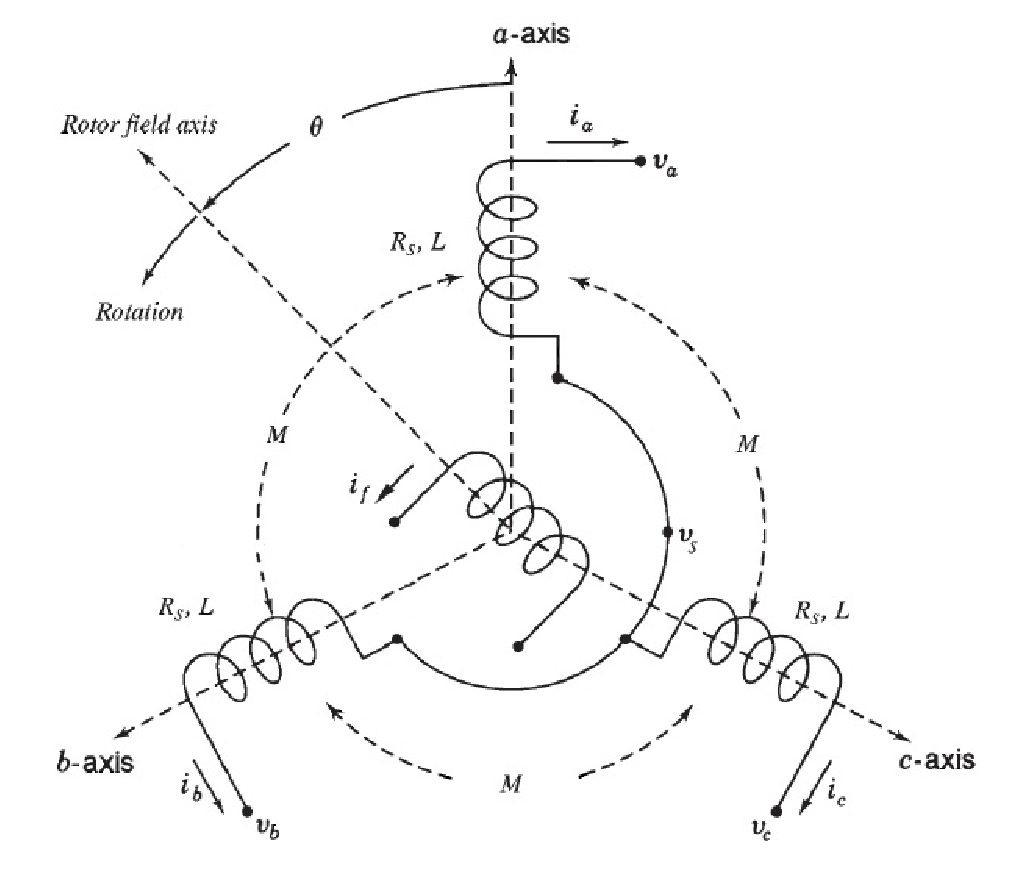
\includegraphics[scale=0.6]{SGStucture}
%\par\end{centering}
%\caption[Structure of an idealized three-phase round rotor synchronous generator]{Structure of an idealized three-phase round rotor synchronous generator,
%modified from \citep{graingerStevenson1994} }
%\end{figure}

The mutual inductance between the rotor coil and the each of the stator
coils varies with the rotor angle $\theta$ as follows:

\[
\left[\begin{array}{c}
M_{a,f}\\
M_{b,f}\\
M_{c,f}
\end{array}\right]=M_{f}\widetilde{\cos}\theta
\]

The flux linkage of the stator windings are

\[
\Phi=\left[\begin{array}{ccc}
L & -M & -M\\
-M & L & -M\\
-M & -M & L
\end{array}\right]i+M_{f}\widetilde{\cos}\theta
\]

The flux of the rotot is:

\begin{equation}
\Phi_{f}=M_{af}i_{a}+M_{bf}i_{b}+M_{cf}i_{c}+L_{f}i_{f}=L_{f}i_{f}+M_{f}<i,\widetilde{\cos}\theta>\label{eq:fieldFlux}
\end{equation}

Because there is no neutral, then $i_{a}+i_{b}+i_{c}=0$, so the previous
equation can be rewritten as 

\[
\Phi=L_{s}i+M_{f}i_{f}\widetilde{\cos}\theta
\]

where $L_{s}=L+M$. Each stator terminal voltage is given by 

\begin{equation}
v=-R_{s}i-\frac{d\Phi}{dt}=-R_{s}i-L_{s}\frac{di}{dt}+e\label{eq:SGTerminalVlotage}
\end{equation}

where $e=\left[\begin{array}{c}
e_{a}\\
e_{b}\\
e_{c}
\end{array}\right]$ is the back electromotive force (EMF) due to the rotor movement given
by:

\begin{equation}
e=M_{f}i_{f}\dot{\theta}\widetilde{\sin}\theta-M_{f}\frac{d\Phi_{f}}{dt}i_{f}\widetilde{\cos}\theta\label{eq:emf}
\end{equation}

And the rotor terminal voltage is given by 

\begin{equation}
v_{f}=-R_{f}i_{f}-\frac{d\Phi_{f}}{dt}\label{eq:fieldVoltage}
\end{equation}

For synchronous generator with no load, the voltages at each terminal
will be sinusoidal function. In order to convert the volteges (and
current) into a fixed value, we will apply Park's transformation:

\[
x_{dq0=}\left[\begin{array}{c}
x_{d}\\
x_{q}\\
x_{0}
\end{array}\right]=U(\theta)\left[\begin{array}{c}
x_{a}\\
x_{b}\\
x_{c}
\end{array}\right]=U(\theta)x_{abc}
\]

where $U(\theta)$ is the unitary matrix:

\begin{equation}
U(\theta)=\sqrt{\frac{3}{2}}\left[\begin{array}{ccc}
\cos(\theta) & \cos(\theta-\frac{2\pi}{3}) & \cos(\theta-\frac{4\pi}{3})\\
\sin(\theta) & \sin(\theta-\frac{2\pi}{3}) & \sin(\theta-\frac{4\pi}{3})\\
\sqrt{\frac{1}{2}} & \sqrt{\frac{1}{2}} & \sqrt{\frac{1}{2}}
\end{array}\right]\label{eq:ParkTransformation}
\end{equation}

where $x_{abc}$ is some vector at abc coordinates, and $x_{dq0}$
is the same vector at the new coordinates.

Applying Park transformation to \eqref{eq:SGTerminalVlotage} leads
to

\begin{equation}
U(\theta)v-U(\theta)e=-R_{s}U(\theta)i-L_{s}U(\theta)\frac{di}{dt}\label{eq:SGTerminalVlotageAfetrPark}
\end{equation}

Using that 

\[
\frac{di_{dq0}}{d\theta}=U(\theta)\frac{di_{abc}}{d\theta}+\frac{dU(\theta)}{d\theta}i_{abc}=U(\theta)\frac{di_{abc}}{d\theta}+\left[\begin{array}{c}
i_{q}\\
-i_{d}\\
0
\end{array}\right]
\]

To calculate the time derivative of $i$:

\[
\dot{i}_{dq0}=\frac{di_{dq0}}{d\theta}\frac{d\theta}{dt}=U(\theta)\dot{i}_{abc}+\omega\left[\begin{array}{c}
i_{q}\\
-i_{d}\\
0
\end{array}\right]
\]

where $\omega=\dot{\theta}$.

We rewrite \eqref{eq:SGTerminalVlotageAfetrPark} as follows:

\begin{equation}
L_{s}\frac{d}{dt}\left[\begin{array}{c}
i_{d}\\
i_{q}\\
i_{0}
\end{array}\right]-L_{s}\omega\left[\begin{array}{c}
i_{q}\\
-i_{d}\\
0
\end{array}\right]=-R_{s}\left[\begin{array}{c}
i_{d}\\
i_{q}\\
i_{0}
\end{array}\right]+\left[\begin{array}{c}
e_{d}-v_{d}\\
e_{q}-v_{q}\\
e_{0}-v_{0}
\end{array}\right]\label{eq:idiqDynamics}
\end{equation}

Because there is no neutral connection, $i_{0}=0,$ hence $e_{0}=0$.
Applying Park transformation on \eqref{eq:emf} gives:

\begin{equation}
\left[\begin{array}{c}
e_{d}\\
e_{q}
\end{array}\right]=-\sqrt{\frac{3}{2}}M_{f}\left[\begin{array}{c}
\frac{di_{f}}{dt}\\
\omega i_{f}
\end{array}\right]\label{eq:ed_eq}
\end{equation}

Substitute \eqref{eq:fieldFlux} into \eqref{eq:fieldVoltage}, and
applying Park's transformation yields:

\[
v_{f}=-R_{f}i_{f}-L_{f}\frac{di_{f}}{dt}-\sqrt{\frac{3}{2}}M_{f}\frac{di_{d}}{dt}
\]

Using \eqref{eq:idiqDynamics} and \eqref{eq:ed_eq} for $\frac{di_{d}}{dt}$
dynamics, and substituting it to the previous equation, gives:

\[
\left(1-\frac{3M_{f}^{2}}{2L_{f}L_{s}}\right)\frac{di_{f}}{dt}=\sqrt{\frac{3}{2}}\frac{M_{f}}{L_{f}}\left(\omega i_{q}-\frac{R_{s}}{L_{s}}i_{d}-\frac{v_{d}}{L_{s}}\right)-\frac{R_{f}}{L_{f}}i_{f}-\frac{v_{f}}{L_{f}}
\]

Denote $\alpha=\left(1-\frac{3M_{f}^{2}}{2L_{f}L_{s}}\right)^{-1}>0$
and $m=\sqrt{\frac{3}{2}}M_{f}$, we have 

\begin{equation}
\frac{di_{f}}{dt}=\frac{\alpha m}{L_{f}}\left(\omega i_{q}-\frac{R_{s}}{L_{s}}i_{d}-\frac{v_{d}}{L_{s}}\right)-\frac{\alpha R_{f}}{L_{f}}i_{f}-\frac{\alpha v_{f}}{L_{f}}\label{eq:if_dynamics}
\end{equation}

Calculate $i_{d}$and $i_{q}$ from \eqref{eq:idiqDynamics} and \eqref{eq:ed_eq},
and substituting $\frac{di_{f}}{dt}$ from \eqref{eq:if_dynamics}
gives:

\begin{equation}
\frac{d}{dt}\left[\begin{array}{c}
i_{d}\\
i_{q}
\end{array}\right]=\omega\left[\begin{array}{c}
i_{q}\\
-i_{d}
\end{array}\right]-\frac{R_{s}}{L_{s}}\left[\begin{array}{c}
i_{d}\\
i_{q}
\end{array}\right]-\frac{m}{L_{s}}\left[\begin{array}{c}
\frac{\alpha m}{L_{f}}\left(\omega i_{q}-\frac{R_{s}}{L_{s}}i_{d}-\frac{v_{d}}{L_{s}}\right)-\frac{\alpha R_{f}}{L_{f}}i_{f}-\frac{\alpha v_{f}}{L_{f}}\\
\omega i_{f}
\end{array}\right]-\left[\begin{array}{c}
v_{d}\\
v_{q}
\end{array}\right]\label{eq:idiqDynamicsWithExIf}
\end{equation}

The rotational dynamics of the rotor is given by the equation:

\begin{equation}
J\dot{\omega}=T_{m}-T_{e}-D_{p}\omega\label{eq:mechanicalPart}
\end{equation}

where $J$ is the moment of inertia of the rotor, $T_{m}$ is is the
mechanical torque which applies by the prime mover, $T_{e}$ is the
electromagnetic torque developed by the generator, and $D_{p}$ is
a damping factor, which consist of the viscous friction acting on
the rotor and the frequency droop from $\omega$ to the mechanical
torque of the prime mover, which added in order to control the frequency
of the generator.

$T_{e}$ can be found from energy consideration. The magnetic energy
stored in the generator is 
\[
E_{mag}=\frac{1}{2}\left(<i,\Phi>+i_{f}\Phi_{f}\right)=\frac{1}{2}\left(<i,L_{s}i>+Li_{f}^{2}\right)+M_{f}i_{f}<i,\widetilde{\cos}\theta>
\]

The electromagnetic torque can be calculated as follows:

\[
T_{e}=\frac{\partial E_{mag}}{\partial\theta}|_{\Phi=const}=\frac{\partial E_{mag}}{\partial\theta}|_{i=const}
\]

\begin{equation}
T_{e}=M_{f}i_{f}<i,\frac{d\tilde{\cos}\theta}{d\theta}>=M_{f}i_{f}<i,\tilde{\sin}\theta>=-mi_{f}i_{q}\label{eq:electricTorque}
\end{equation}

Using \eqref{eq:idiqDynamicsWithExIf}, \eqref{eq:if_dynamics}, \eqref{eq:mechanicalPart}
and \eqref{eq:electricTorque} we obtained:
\begin{equation}
\begin{array}{ccc}
\frac{d}{dt}\left[\begin{array}{c}
L_{s}i_{d}\\
L_{s}i_{q}\\
L_{f}i_{f}\\
J\omega
\end{array}\right] & = & \left[\begin{array}{cccc}
-\alpha R_{s} & \alpha\omega L_{s} & \alpha mR_{f} & 0\\
-\omega L_{s} & -R_{s} & 0 & -mi_{f}\\
\frac{\alpha mR_{s}}{L_{s}} & -\alpha m\omega & -\alpha R_{f} & 0\\
0 & mi_{f} & 0 & -D_{p}
\end{array}\right]\left[\begin{array}{c}
i_{d}\\
i_{q}\\
i_{f}\\
\omega
\end{array}\right]\\
 & + & \left[\begin{array}{cccc}
-\alpha & 0 & \frac{\alpha m}{L_{f}} & 0\\
0 & -1 & 0 & 0\\
\frac{\alpha m}{L_{s}} & 0 & -\alpha & 0\\
0 & 0 & 0 & 1
\end{array}\right]\left[\begin{array}{c}
v_{d}\\
v_{q}\\
v_{f}\\
T_{m}
\end{array}\right]
\end{array}
\end{equation}

This fourth order nonlinear dynamical system represents the dynamics
of single SG. 

\section{Single generator with constant field current dynamics}

At this sections, we assume that the rotor current is constant (which
means that the field dynamics is very fast, or equivalently, the rotor
is composed of permanent magnet).

Assuming $\frac{di_{f}}{dt}=0$, and substituting it at \eqref{eq:idiqDynamicsWithExIf}
gives:

\begin{equation}
\frac{d}{dt}\left[\begin{array}{c}
i_{d}\\
i_{q}
\end{array}\right]=\omega\left[\begin{array}{c}
i_{q}\\
-i_{d}
\end{array}\right]-\frac{R_{s}}{L_{s}}\left[\begin{array}{c}
i_{d}\\
i_{q}
\end{array}\right]-\frac{m}{L_{s}}\left[\begin{array}{c}
0\\
\omega i_{f}
\end{array}\right]-\left[\begin{array}{c}
v_{d}\\
v_{q}
\end{array}\right]\label{eq:idiqDynamicsWithFixxIf}
\end{equation}

Using \eqref{eq:idiqDynamicsWithFixxIf}, \eqref{eq:mechanicalPart}
and \eqref{eq:electricTorque} we obtained:

\begin{equation}
\frac{d}{dt}\left[\begin{array}{c}
L_{s}i_{d}\\
L_{s}i_{q}\\
J\omega
\end{array}\right]=\left[\begin{array}{ccc}
-R_{s} & \omega L_{s} & 0\\
-\omega L_{s} & -R_{s} & -mi_{f}\\
0 & mi_{f} & -D_{p}
\end{array}\right]\left[\begin{array}{c}
i_{d}\\
i_{q}\\
\omega
\end{array}\right]+\left[\begin{array}{c}
-v_{d}\\
-v_{q}\\
T_{m}
\end{array}\right]\label{eq:SGDynamics}
\end{equation}

This Third order nonlinear dynamical system represents the dynamics
of single SG with constant field current. 

\section{Model of a single generator connected to an infinite bus }

In this section we develop a model for single synchronous generator
which connected to an infinite bus. This section follows \citep{NatarajanWeiss2015}.
The infinite bus is model as tree phase AC voltage source. i.e the
infinite bus is not effected by the synchronous generator that connected
to it. The reason for this model is that the influence of a single
synchronous generator on a grid is very small. In general, the line
that connect the synchronous generator to the grid has its impedance
that consist of resistance and inductance, but because it connected
to the synchronous generator in series, then the $R_{s}$ and $L_{s}$
parameters can take into account the impedance of both the synchronous
generator and the line.

Because the infinite bus is modeled as voltage source, then the voltage
at the synchronous generator terminals is

\begin{equation}
v=\left[\begin{array}{c}
v_{a}\\
v_{b}\\
v_{c}
\end{array}\right]=\sqrt{\frac{2}{3}}V\left[\begin{array}{c}
\cos(\theta_{g})\\
\cos(\theta_{g}-\frac{2\pi}{3})\\
\cos(\theta_{g}-\frac{4\pi}{3})
\end{array}\right]\label{eq:infBusVoltageABC}
\end{equation}

where $V$ is the grid voltage magnitude, and $\theta_{g}$ is the
grid phase. Lets define the angle $\delta$ which represent the difference
between the grid and the synchronous generator angles:

\[
\delta=\theta-\theta_{g}
\]

After applying Park transformation (which depends on $\theta$ which
is the synchronous generator phase) on \eqref{eq:infBusVoltageABC}
we have 

\begin{equation}
v_{dqo}=\left[\begin{array}{c}
v_{d}\\
v_{q}\\
v_{0}
\end{array}\right]=U(\theta)\sqrt{\frac{2}{3}}V\left[\begin{array}{c}
\cos(\theta_{g})\\
\cos(\theta_{g}-\frac{2\pi}{3})\\
\cos(\theta_{g}-\frac{4\pi}{3})
\end{array}\right]=-V\left[\begin{array}{c}
\sin(\delta)\\
\cos(\delta)\\
0
\end{array}\right]\label{eq:infBusVoltageDQO}
\end{equation}

It is easy to see that the dynamics of $\delta$ is 

\begin{equation}
\dot{\delta}=\omega-\omega_{g}\label{eq:deltaDynamics}
\end{equation}

where $\omega_{g}$ is the grid frequency. Substituting \eqref{eq:infBusVoltageDQO}
and \eqref{eq:deltaDynamics} into \eqref{eq:SGDynamics} gives:

\begin{equation}
\frac{d}{dt}\left[\begin{array}{c}
L_{s}i_{d}\\
L_{s}i_{q}\\
J\omega\\
\delta
\end{array}\right]=\left[\begin{array}{cccc}
-R_{s} & \omega L_{s} & 0 & 0\\
-\omega L_{s} & -R_{s} & -mi_{f} & 0\\
0 & mi_{f} & -D_{p} & 0\\
0 & 0 & 1 & 0
\end{array}\right]\left[\begin{array}{c}
i_{d}\\
i_{q}\\
\omega\\
\delta
\end{array}\right]+\left[\begin{array}{c}
V\sin(\delta)\\
V\cos(\delta)\\
T_{m}\\
\omega_{g}
\end{array}\right]\label{eq:SGDynamicsInfBus}
\end{equation}

This fourth order nonlinear dynamical system is the model for one
synchronous generator which connected to an infinite bus.

\section{Model of microgrid comprising two synchronous generators in parallel}

In this section, we consider a microgrid comprising two identical
synchronous generators, with constant rotor (field) current and no
neutral connection, together with a resistive load (see Figure \ref{fig:microgrid_configuration}).

\begin{figure}
\begin{circuitikz}[american voltages]
\begin{scope}[shift={(-5,0)}]     \draw (0,0) node[anchor=east] {0} to [L=Z, *-o] (90 :2.5) node[anchor=east]{$v_a$}; \draw (0,0) to [L=Z, *-o] (210 :2.5) node[anchor=east]{$v_b$}; \draw (0,0) to [L=Z, *-o] (330 :2.5) node[anchor=east]{$v_c$}; \node (0,0) [align=left,text width=4cm] {SG1}; \end{scope}
   \draw (0,0) node[anchor=east] {0} to [R=$R_L$, *-o] (90 :2.5) node[anchor=east]{}; \draw (0,0) to [R=$R_L$] (210 :2.5); \draw (0,0) to [R=$R_L$] (330 :2.5);
\begin{scope}[shift={(5,0)}]    \draw (0,0) node[anchor=east] {0} to [L=Z, *-o] (90 :2.5) node[anchor=west] {$v_a$}; \draw (0,0) to [L=Z, *-o] (210 :2.5) node[anchor=east]{$v_b$}; \draw (0,0) to [L=Z, *-o] (330 :2.5) node[anchor=east]{$v_c$}; \node (0,0) [align=left,text width=4cm] {SG2}; \end{scope}
\draw (5,2.5) to [short, i>=$i_{a2}$] (0,2.5) to [short, i<=$i_{a1}$] (-5,2.5); \draw (-2.165 +5,-1.25) to [short] (-2.165 +5,-1.25 -1) to [short, i>=$i_{b2}$]   (-2.165 ,-1.25-1)  to [short, o-] (-2.165 ,-1.25 ); \draw (-2.165 -5,-1.25) to [short] (-2.165 -5,-1.25 -1) to [short, i>=$i_{b1}$]   (-2.165 ,-1.25-1); \draw (2.165 +5,-1.25) to [short] (2.165 +5,-1.25 -2) to [short, i>=$i_{c2}$]  (2.165 ,-1.25-2)  to [short, o-] (2.165 ,-1.25 ); \draw (2.165 -5,-1.25) to [short] (2.165 -5,-1.25 -2) to [short, i>=$i_{c1}$]  (2.165 ,-1.25-2);
\end{circuitikz}\caption{Microgrid comprising two synchronous generators configuration}

\label{fig:microgrid_configuration}
\end{figure}

The rotor angles are $\theta_{1}$ and $\theta_{2}$ and the torques
acting on the generators are equal, denoted $T_{m}$. By symmetry,
we assume that the voltages at the (non-connected) midpoints of the
generators and the load are zero.

The phase voltages and currents are:

\[
v_{1}=\left[\begin{array}{c}
v_{a1}\\
v_{b1}\\
v_{c1}
\end{array}\right],\quad v_{2}=\left[\begin{array}{c}
v_{a2}\\
v_{b2}\\
v_{c2}
\end{array}\right],\quad i_{1}=\left[\begin{array}{c}
i_{a1}\\
i_{b1}\\
i_{c1}
\end{array}\right],\quad i_{2}=\left[\begin{array}{c}
i_{a2}\\
i_{b2}\\
i_{c2}
\end{array}\right]
\]

The impedances $Z=R_{s}+R_{g}+(L_{s}+L_{g})s$ are comprised of the
equivalent stator resistance $R_{s}$ and stator inductance $L_{s}$
and the line resistance $R_{g}$ and inductance $L_{g}$. However,
we consider for simplicity that $R_{g}=0$ and $L_{g}=0$, since this
leaves us with the same type of equations, see Figure \ref{fig:one_phase_scheme}.

\begin{figure}
\begin{circuitikz}[american voltages] \draw   (0,0) node[ground] {}   to [V,v=$e_{j1}$] (0,3) {}   to [R=$R_s$,i>=$i_{j1}$] (3,3){}   to [L=$L_s$] (5,3){}   to [R=$R_L$, o-] (5,0){}    to  (5,0) node[ground] {};   \draw   (10,0) node[ground] {}   to [V,v=$e_{j2}$] (10,3) {}   to [R=$R_s$,i>=$i_{j2}$] (7,3){}   to [L=$L_s$] (5,3){};   \node[draw] at (-1,4) {$j \in \{a,b,c\}$}; \end{circuitikz} 

\caption{Microgrid comprising two synchronous generators one phase scheme}

\label{fig:one_phase_scheme}
\end{figure}

Recall Park transformation \eqref{eq:ParkTransformation}, and apply
it on the currents and voltages we have:

\[
\left[\begin{array}{c}
v_{d1}\\
v_{q1}\\
v_{01}
\end{array}\right]=U(\theta_{1})\left[\begin{array}{c}
v_{a1}\\
v_{b1}\\
v_{c1}
\end{array}\right],\quad\left[\begin{array}{c}
v_{d2}\\
v_{q2}\\
v_{02}
\end{array}\right]=U(\theta_{2})\left[\begin{array}{c}
v_{a2}\\
v_{b2}\\
v_{c2}
\end{array}\right]
\]

\[
\left[\begin{array}{c}
i_{d1}\\
i_{q1}\\
i_{01}
\end{array}\right]=U(\theta_{1})\left[\begin{array}{c}
i_{a1}\\
i_{b1}\\
i_{c1}
\end{array}\right],\quad\left[\begin{array}{c}
i_{d2}\\
i_{q2}\\
i_{02}
\end{array}\right]=U(\theta_{2})\left[\begin{array}{c}
i_{a2}\\
i_{b2}\\
i_{c2}
\end{array}\right]
\]

Clearly $i_{01}=i_{02}=0$ (from Kirchhoff's laws) and by symmetry
argument we can show that $v_{01}=v_{02}=0$ (because $v_{a}=R_{L}(i_{a1}+i_{a2})$
etc).

Thus, we only have to deal with $v_{dj},v_{qj}$ (with $j\in\{1,2\}$). 

We denote 

\[
\delta=\theta_{2}-\theta_{1}
\]

According to formula \eqref{eq:SGDynamics}, the dynamics of synchronous
machine:

\begin{equation}
\frac{d}{dt}\left[\begin{array}{c}
L_{s}i_{d1}\\
L_{s}i_{q1}\\
J\omega_{1}
\end{array}\right]=\left[\begin{array}{ccc}
-R_{s} & \omega_{1}L_{s} & 0\\
-\omega_{1}L_{s} & -R_{s} & -mi_{f}\\
0 & mi_{f} & D_{p}
\end{array}\right]\left[\begin{array}{c}
i_{d1}\\
i_{q1}\\
\omega_{1}
\end{array}\right]+\left[\begin{array}{c}
-v_{d1}\\
-v_{q1}\\
T_{m}
\end{array}\right]\label{eq:dynamics_of_single_generator}
\end{equation}

where $J$ is the moment of inertia, $D_{p}$ is the frequency droop
constant, $T_{m}$ is the mechanical torque coming from the prime
mover to the generator, $m=\sqrt{\frac{3}{2}}M_{f}$, where $M_{f}$
is the peak mutual inductance between the rotor and one of the stator
windings, and $i_{f}$ is the rotor current. Of course, a similar
equation holds for the second generator. To put the equations together,
we use 

\[
v=R_{L}(i_{1}+i_{2})
\]

and after applying Park transformation:

\[
\left[\begin{array}{c}
v_{d1}\\
v_{q1}\\
0
\end{array}\right]=R_{L}\left[\begin{array}{c}
i_{d1}\\
i_{q1}\\
0
\end{array}\right]+R_{L}U(\theta_{1})\left[\begin{array}{c}
i_{a2}\\
i_{b2}\\
i_{c2}
\end{array}\right]
\]

\begin{equation}
\left[\begin{array}{c}
v_{d1}\\
v_{q1}\\
0
\end{array}\right]=R_{L}\left[\begin{array}{c}
i_{d1}\\
i_{q1}\\
0
\end{array}\right]+R_{L}U(\theta_{1})U(\theta_{2})^{-1}\left[\begin{array}{c}
i_{d2}\\
i_{q2}\\
0
\end{array}\right]\label{eq:cur_and_volt_after_park}
\end{equation}

A simple computation shows that 

\[
U(\theta_{1})U(\theta_{2})^{-1}=\left[\begin{array}{ccc}
\cos(\delta) & -\sin(\delta) & 0\\
\sin(\delta) & \cos(\delta) & 0\\
0 & 0 & 1
\end{array}\right]
\]

(recall that $\delta=\theta_{2}-\theta_{1}$).

now, substitute that at \eqref{eq:cur_and_volt_after_park} gives:

\[
\left[\begin{array}{c}
v_{d1}\\
v_{q1}
\end{array}\right]=R_{L}\left[\begin{array}{c}
i_{d1}\\
i_{q1}
\end{array}\right]+R_{L}\left[\begin{array}{cc}
\cos(\delta) & -\sin(\delta)\\
\sin(\delta) & \cos(\delta)
\end{array}\right]\left[\begin{array}{c}
i_{d2}\\
i_{q2}
\end{array}\right]
\]

Substituting this into \eqref{eq:dynamics_of_single_generator}, denoting
$R_{tot}=R_{s}+R_{L}$:

\begin{equation}
\begin{array}{ccc}
\frac{d}{dt}\left[\begin{array}{c}
L_{s}i_{d1}\\
L_{s}i_{q1}\\
J\omega_{1}
\end{array}\right] & = & \left[\begin{array}{ccc}
-R_{tot} & \omega_{1}L_{s} & 0\\
-\omega_{1}L_{s} & -R_{tot} & -mi_{f}\\
0 & mi_{f} & D_{p}
\end{array}\right]\left[\begin{array}{c}
i_{d1}\\
i_{q1}\\
\omega_{1}
\end{array}\right]+\left[\begin{array}{c}
0\\
0\\
T_{m}
\end{array}\right]\\
 &  & -\left[\begin{array}{ccc}
R_{L}\cos(\delta) & -R_{L}\sin(\delta) & 0\\
R_{L}\sin(\delta) & R_{L}\cos(\delta) & 0\\
0 & 0 & 0
\end{array}\right]\left[\begin{array}{c}
i_{d2}\\
i_{q2}\\
\omega_{2}
\end{array}\right]
\end{array}\label{dynamics_of_microgrid}
\end{equation}

or in short:

\[
\varLambda\dot{z}_{1}=\mathcal{A}(\omega_{1})z_{1}+T_{m}e_{3}-\mathcal{B}(\delta)z_{2}
\]

Where 

\[
\varLambda=\left[\begin{array}{ccc}
L_{s} & 0 & 0\\
0 & L_{s} & 0\\
0 & 0 & J
\end{array}\right],e_{3}=\left[\begin{array}{c}
0\\
0\\
1
\end{array}\right]
\]

\[
\mathcal{A}(\omega)=\left[\begin{array}{ccc}
-R_{tot} & \omega L_{s} & 0\\
-\omega L_{s} & -R_{tot} & -mi_{f}\\
0 & mi_{f} & D_{p}
\end{array}\right],\mathcal{B}(\delta)=\left[\begin{array}{ccc}
R_{L}\cos(\delta) & -R_{L}\sin(\delta) & 0\\
R_{L}\sin(\delta) & R_{L}\cos(\delta) & 0\\
0 & 0 & 0
\end{array}\right]
\]

\[
,z_{i}=\left[\begin{array}{c}
i_{di}\\
i_{qi}\\
\omega_{i}
\end{array}\right],i\in\{1,2\}
\]

Of course a symmetric equation holds for the second generator:

\[
\varLambda\dot{z}_{2}=\mathcal{A}(\omega_{2})z_{2}+T_{m}e_{3}-\mathcal{B}(-\delta)z_{1}
\]

There is a seventh state variable, $\delta$, for which the ODE is 

\[
\dot{\delta}=\omega_{2}-\omega_{1}
\]

The whole system is described by:

\begin{equation}
\frac{d}{dt}\left[\begin{array}{c}
\varLambda z_{1}\\
\varLambda z_{2}\\
\delta
\end{array}\right]=\left[\begin{array}{c|c|c}
\mathcal{A}(\omega_{1}) & -\mathcal{B}(\delta) & 0\\
\hline -\mathcal{B}(-\delta) & \mathcal{A}(\omega_{2}) & 0\\
\hline -e_{3}^{T} & e_{3}^{T} & 0
\end{array}\right]\left[\begin{array}{c}
z_{1}\\
z_{2}\\
\delta
\end{array}\right]+T_{m}\left[\begin{array}{c}
e_{3}\\
e_{3}\\
0
\end{array}\right]\label{eq:dynamics_whole}
\end{equation}




\chapter{Equilibrium points \label{cha:equivalence_pont}}

In this chapter, we study the equilibrium points for both the infinite
bus configuration, and the two SG microgid.

\section{Equilibrium points of SG connected to an infinite bus.}

This section follows \citep{NatarajanWeiss2015}. In order to search
the equilibrium point of single SG which connected to an infinite
bus, we will find the roots of: 

\begin{equation}
\left[\begin{array}{c}
0\\
0\\
0\\
0
\end{array}\right]=\left[\begin{array}{cccc}
-R_{s} & \omega^{e}L_{s} & 0 & 0\\
-\omega^{e}L_{s} & -R_{s} & -mi_{f} & 0\\
0 & mi_{f} & -D_{p} & 0\\
0 & 0 & 1 & 0
\end{array}\right]\left[\begin{array}{c}
i_{d}^{e}\\
i_{q}^{e}\\
\omega^{e}\\
\delta^{e}
\end{array}\right]+\left[\begin{array}{c}
V\sin\delta^{e}\\
V\cos\delta^{e}\\
T_{m}\\
\omega_{g}
\end{array}\right]\label{eq:SGDynamicsInfBusEqPoint}
\end{equation}

By taking the fourth, and the third lines, it shows that the equilibrium
point $z_{e}=\left[\begin{array}{c}
i_{d}^{e}\\
i_{q}^{e}\\
\omega^{e}\\
\delta^{e}
\end{array}\right]$ must satisfy:

\[
\omega^{e}=\omega_{g},\qquad i_{q}^{e}=\frac{D_{p}\omega_{g}-T_{m}}{mi_{f}}
\]

Using the value of $i_{q}^{e}$ at the first line yields:

\[
i_{d}^{e}=\frac{\omega_{g}L_{s}\left(D_{p}\omega_{g}-Tm\right)}{mi_{f}R_{s}}+\frac{V\sin\delta^{e}}{R_{s}}
\]

Using the second line, after substituting the values of $i_{d}^{e}$
and $i_{q}^{e}$ gives:

\[
\delta^{e}=\cos^{-1}\left(\frac{mi_{f}\omega_{g}R_{s}}{|Z|V}-\frac{|z|\left(T_{m}D_{p}\omega_{g}\right)}{Vmi_{f}}\right)-\psi
\]

where $|z|$ and $\psi$ define by the impedance of the generator:
$z=R_{s}+j\omega_{g}L_{s}=|z|e^{j\psi}$.

Because the arccos function, SG which connected to an infinite bus
can have one, two or zero solutions (modulo $2\pi$).

\section{Equilibrium points of a microgrid comprising two SGs.}

In this section, we study the equilibrium points of a microgrid domprising
two SGs. We start by showing that such equilibrium point must satisfy
synchronization between the two generators (means that the state variables
are equal between the two generators, and there is no phase between
the two generators), or anti-synchronization between the two generators
(means that the state variables are equal between the two generators,
and there is phase of $\pi$ between the two generators). Later in
this section, we show that there exist at list one equilibrium point,
which located on the manifold of synchronization of the two generators. 

\subsection{An equilibrium can be only on the surface $z_{1}=z_{2}$.}

First, we will show that the system \eqref{eq:dynamics_whole} has
equilibrium point, and those equilibrium point have the structure
$z_{1}^{e}=z_{2}^{e}=z^{e},\qquad\delta^{e}=\pi k,\qquad k\in\mathbb{Z}$.
For proving that, we will start form the algebraic equation:

\[
\left[\begin{array}{c|c|c}
\mathcal{A}(\omega_{1}^{e}) & -\mathcal{B}(\delta^{e}) & 0\\
\hline -\mathcal{B}(-\delta^{e}) & \mathcal{A}(\omega_{2}^{e}) & 0\\
\hline -e_{3}^{T} & e_{3}^{T} & 0
\end{array}\right]\left[\begin{array}{c}
z_{1}^{e}\\
z_{2}^{e}\\
\delta^{e}
\end{array}\right]+T_{m}\left[\begin{array}{c}
e_{3}\\
e_{3}\\
0
\end{array}\right]=0
\]

At the seventh line ($\dot{\delta})$ we have 
\[
-\omega_{1}^{e}+\omega_{2}^{e}=0\longrightarrow\omega_{1}^{e}=\omega_{2}^{e}\coloneqq\omega^{e}
\]

From the third line ($\dot{\omega}_{1})$ and the sixth line ($\dot{\omega}_{2})$
we have 

\[
\left\{ \begin{array}{c}
mi_{f}i_{q1}^{e}-D_{p}\omega_{1}^{e}+T_{m}=0\\
mi_{f}i_{q2}^{e}-D_{p}\omega_{2}^{e}+T_{m}=0
\end{array}\right.\longrightarrow\left\{ \begin{array}{c}
mi_{f}i_{q1}^{e}-D_{p}\omega^{e}=0\\
mi_{f}i_{q2}^{e}-D_{p}\omega^{e}=0
\end{array}\right.\longrightarrow i_{q1}^{e}=i_{q2}^{e}=i_{q}^{e}
\]

From the first line ($\dot{i}_{d1})$, the second line ($\dot{i}_{q1})$,
the forth line ($\dot{i}_{d2})$ and the fifth line ($\dot{i}_{q2})$
we have 

\[
\left\{ \begin{array}{c}
-R_{tot}i_{d1}^{e}+\omega^{e}L_{s}i_{q}^{e}-R_{L}\cos\delta^{e}i_{d2}^{e}+R_{L}\sin\delta^{e}i_{q}^{e}=0\\
-\omega^{e}L_{s}i_{d1}^{e}-R_{tot}i_{q}^{e}-mi_{f}\omega^{e}-R_{L}\sin\delta^{e}i_{d2}^{e}-R_{L}\cos\delta^{e}i_{q}^{e}=0\\
-R_{tot}i_{d2}^{e}+\omega^{e}L_{s}i_{q}^{e}-R_{L}\cos\delta^{e}i_{d1}^{e}-R_{L}\sin\delta^{e}i_{q}^{e}=0\\
-\omega^{e}L_{s}i_{d2}^{e}-R_{tot}i_{q}^{e}-mi_{f}\omega^{e}+R_{L}\sin\delta^{e}i_{d1}^{e}-R_{L}\cos\delta^{e}i_{q}^{e}=0
\end{array}\right.
\]

This system of equations can be represented at matrix form:

\begin{equation}
M\left[\begin{array}{c}
i_{d1}^{e}\\
i_{d2}^{e}
\end{array}\right]=n\label{eq:equilibrium_system}
\end{equation}

Where 

\[
M=\left[\begin{array}{cc}
-R_{tot} & -R_{L}\cos\delta^{e}\\
-\omega^{e}L_{s} & -R_{L}\sin\delta^{e}\\
-R_{L}\cos\delta^{e} & -R_{tot}\\
R_{L}\sin\delta^{e} & -\omega^{e}L_{s}
\end{array}\right]
\]

and 

\[
n=\left[\begin{array}{c}
i_{q}^{e}\left(\omega^{e}L_{s}+R_{L}\sin\delta^{e}\right)\\
-mi_{f}\omega^{e}-i_{q}^{e}\left(R_{tot}+R_{L}\cos\delta^{e}\right)\\
i_{q}^{e}\left(\omega^{e}L_{s}-R_{L}\sin\delta^{e}\right)\\
-mi_{f}\omega^{e}-i_{q}^{e}\left(R_{tot}+R_{L}\cos\delta^{e}\right)
\end{array}\right]
\]


\subparagraph*{Rouché\textendash Capelli Theorem: }

The system $Mx=n$ has a solution if and only if $rank\left[M|n\right]=rank\left[M\right].$

We will prove by contradiction that $\sin\delta_{0}=0$ is a necessary
condition for the system \eqref{eq:equilibrium_system} to have solution.
Negated to assume that $\sin\delta^{e}\ne0$. We will show that $rank\left[M|n\right]=3.$

Denote $\alpha=\omega_{0}L_{s}+R_{L}\sin\delta_{0}$ and $\beta=\omega_{0}L_{s}-R_{L}\sin\delta_{0}$,
then:

\begin{equation}
\left[M|n\right]=\left[\begin{array}{ccc}
-R_{tot} & \quad-R_{L}\cos\delta^{e}\quad & i_{q}^{e}\alpha\\
-\omega^{e}L_{s} & \quad-R_{L}\sin\delta^{e}\quad & -mi_{f}\omega^{e}-i_{q}^{0}\left(R_{tot}+R_{L}\cos\delta^{e}\right)\\
-R_{L}\cos\delta^{e} & \quad-R_{tot}\quad & i_{q}^{e}\beta\\
R_{L}\sin\delta^{e} & \quad-\omega^{e}L_{s}\quad & -mi_{f}\omega^{e}-i_{q}^{0}\left(R_{tot}+R_{L}\cos\delta^{e}\right)
\end{array}\right]\label{eq:M_n}
\end{equation}


\subsubsection*{Case A: $\alpha=0$ and $\beta=0$}

Because $\alpha=0$ and $\beta=0$ it means that $\omega^{e}L_{s}+R_{L}\sin\delta^{e}=\omega^{e}L_{s}-R_{L}\sin\delta^{e}$
hance $R_{L}\sin\delta^{e}=0$ which contradicts our assumption.

\subsubsection*{Case B: $\alpha=0$ and $\beta\protect\ne0$}

Lets define 

\begin{equation}
T=\left[\begin{array}{cccc}
0 & 0 & 1 & 0\\
1 & 0 & 0 & 0\\
0 & 1 & 0 & -1
\end{array}\right]\left[M|n\right]=\left[\begin{array}{ccc}
-R_{L}\cos\delta^{e} & -R_{tot} & i_{q}^{e}\beta\\
-R_{tot} & -R_{L}\cos\delta^{e} & 0\\
0 & \beta & 0
\end{array}\right]\label{eq:MATRIX_1}
\end{equation}

Now, if $\cos\delta^{e}=0$ then $rank(T)=3$. If $\cos\delta^{e}\ne0$
we define 

\[
T_{2}=\left[\begin{array}{ccc}
1 & 0 & 0\\
0 & \beta & -R_{L}\cos\delta^{e}\\
0 & 0 & 1
\end{array}\right]T=\left[\begin{array}{ccc}
-R_{L}\cos\delta_{0} & -R_{tot} & i_{q}^{e}\beta\\
-R_{tot}\beta & 0 & 0\\
0 & \beta & 0
\end{array}\right]
\]

it is easy to see that $rank(T_{2})=3$.

\subsubsection*{Case C: $\alpha\protect\ne0$ and $\beta=0$}

Lets define

\begin{equation}
T_{3}=\left[\begin{array}{cccc}
1 & 0 & 0 & 0\\
0 & 0 & 1 & 0\\
0 & 1 & 0 & -1
\end{array}\right]\left[M|n\right]=\left[\begin{array}{ccc}
-R_{tot} & -R_{L}\cos\delta^{e} & i_{q}^{e}\alpha\\
-R_{L}\cos\delta^{e} & -R_{tot} & 0\\
-\alpha & 0 & 0
\end{array}\right]\label{eq:MATRIX_2}
\end{equation}

it is easy to see that $rank(T_{3})=3$.

\subsubsection*{Case D: $\alpha\protect\ne0$ and $\beta\protect\ne0$}

Lets define

\begin{equation}
T_{4}=\left[\begin{array}{cccc}
1 & 0 & 0 & 0\\
\alpha & 0 & \beta & 0\\
0 & 1 & 0 & -1
\end{array}\right]\left[M|n\right]=\left[\begin{array}{ccc}
-R_{tot} & -R_{L}\cos\delta^{e} & i_{q}^{e}\alpha\\
\frac{R_{L}\cos\delta^{e}}{\beta}-\frac{R_{tot}}{\alpha} & -\frac{R_{L}\cos\delta^{e}}{\alpha}+\frac{R_{tot}}{\beta} & 0\\
-\alpha & \beta & 0
\end{array}\right]\label{eq:MATRIX_4}
\end{equation}

Now, if $-\frac{R_{L}\cos\delta_{0}}{\alpha}+\frac{R_{tot}}{\beta}=0$,
because $\frac{R_{L}\cos\delta^{e}}{\beta}-\frac{R_{tot}}{\alpha}$
must be different than zero, it is easy to see that $rank(T_{4})=3$.
(It is impossible that both $-\frac{R_{L}\cos\delta^{e}}{\alpha}+\frac{R_{tot}}{\beta}=0$
and $\frac{R_{L}\cos\delta^{e}}{\beta}-\frac{R_{tot}}{\alpha}=0$
because that implies that $(\alpha+\beta)R_{L}\cos\delta^{e}=(\alpha+\beta)R_{tot}$,
and $\alpha+\beta=2\omega^{e}L_{s}>0$ and $R_{tot}>R_{L}\cos\delta^{e}$).

Assuming that $-\frac{R_{L}\cos\delta_{0}}{\alpha}+\frac{R_{tot}}{\beta}\ne0$
we define

\[
\begin{array}{c}
T_{5}=\left[\begin{array}{ccc}
1 & 0\quad & 0\\
0 & 0\quad & 1\\
0 & -\frac{R_{L}\cos\delta_{0}}{\alpha}+\frac{R_{tot}}{\beta}\quad & -\beta
\end{array}\right]T_{4}=\\
\left[\begin{array}{ccc}
-R_{tot} & -R_{L}\cos\delta^{e} & i_{q}^{e}\alpha\\
-\alpha & \beta & 0\\
\frac{4L_{s}R_{tot}\omega^{e}\sin\delta^{e}}{\beta\left[L_{s}\omega^{0}\left(R_{tot}-R_{L}\cos\delta^{e}\right)+R_{L}\left(R_{tot}+R_{L}\cos\delta^{e}\right)\sin\delta^{0}\right]} & 0 & 0
\end{array}\right]
\end{array}
\]

by assumption, $\sin\delta^{e}\ne0$ which imply that $rank(T_{5})=3$. 

Because we showed that for any possible case, after applying linear
transformation on $\left[M|n\right]$ the resulting rank is 3, it
implies that $rank\left[M|n\right]=3.$ 

Obviously, $rank\left[M\right]\le2$ which implies that under the
assumption that $\sin\delta^{e}\ne0$ the system \eqref{eq:equilibrium_system}
doesn't have solution. That means that if there is equilibrium point
for the system \eqref{eq:dynamics_whole}, it must satisfied $\sin\delta^{e}=0$
which means that $\delta^{e}=\pi k,\qquad k\in\mathbb{Z}.$

If $\delta^{e}=\pi k,\qquad k\in\mathbb{Z}$ then $\sin\delta^{e}=0$
and $\cos\delta^{e}=1$.Now: 

\[
M=\left[\begin{array}{cc}
-R_{tot} & -R_{L}\\
-\omega^{e}L_{s} & 0\\
-R_{L} & -R_{tot}\\
0 & -\omega^{e}L_{s}
\end{array}\right]
\]

and 

\[
N=\left[\begin{array}{c}
i_{q}^{e}\omega^{e}L_{s}\\
-mi_{f}\omega^{e}-i_{q}^{e}\left(R_{tot}+R_{L}\right)\\
i_{q}^{e}\omega^{e}L_{s}\\
-mi_{f}\omega^{e}-i_{q}^{e}\left(R_{tot}+R_{L}\right)
\end{array}\right]
\]

This system have one solution: $i_{d1}^{e}=i_{d2}^{e}\coloneqq i_{d}^{e}$

\subsection{Equilibrium point on the synchronization surface.}

The algebraic equation for calculating $z^{e}=z_{1}^{e}=z_{2}^{e}$
is:

\begin{equation}
\left[\begin{array}{ccc}
-R_{s}-2R_{L} & \omega^{e}L_{s} & 0\\
-\omega^{e}L_{s} & -R_{s}-2R_{L} & -mi_{f}\\
0 & mi_{f} & -D_{p}
\end{array}\right]\left[\begin{array}{c}
i_{d}^{e}\\
i_{q}^{e}\\
\omega^{e}
\end{array}\right]=\left[\begin{array}{c}
0\\
0\\
-T_{m}
\end{array}\right]\label{eq:equilbrium_algebric_eq}
\end{equation}

We take scalar products on both sides with $z^{e}$:

\[
\left(R_{tot}+R_{L}\right)\left((i_{d}^{e})^{2}+(i_{q}^{e})^{2}\right)=\left(T_{m}-D_{p}\omega^{e}\right)\omega^{e}
\]

This equation makes perfect physical sense. Indeed, assume that there
is no actual friction in the machine, $D_{p}$ is created by feedback,
so that $T_{m}-D_{p}\omega^{e}$ is the mechanical torque applied
to one generator, and then $\left(T_{m}-D_{p}\omega^{e}\right)\omega^{e}$
is the mechanical power entering one generator. On the other hand,
it is easy to see that $\left(R_{tot}+R_{L}\right)\left((i_{d}^{e})^{2}+(i_{q}^{e})^{2}\right)=\left(R_{s}+2R_{L}\right)\left(i_{a}^{2}+i_{b}^{2}+i_{c}^{2}\right)$
which is exactly half of the power dissipated in all the resistors,
hence it is the electric power leaving one generator.

From \eqref{eq:equilbrium_algebric_eq}, we want to derive a scalar
equation to the determine the equilibrium velocity $\omega^{0}$.
The last line of the matrix equation \eqref{eq:equilbrium_algebric_eq}
is $mi_{f}i_{q}^{e}-D_{p}\omega^{e}=-T_{m}$. from where

\begin{equation}
T_{m}-D_{p}\omega^{e}=-mi_{f}i_{q}^{e}\label{eq:eq_0_first_eq}
\end{equation}

The sides of this equation are the mechanical torque acting on each
generator at equilibrium.

The first line of the matrix equilibrium \eqref{eq:equilbrium_algebric_eq}
is $-\left(R_{tot}+R_{L}\right)i_{d}^{e}+\omega^{e}L_{tot}i_{q}^{e}=0$,
hence:

\[
i_{d}^{e}=\frac{\omega^{e}L_{s}}{R_{tot}+R_{L}}i_{q}^{e}
\]

From \eqref{eq:eq_0_first_eq} 
\begin{equation}
i_{q}^{e}=\frac{T_{m}-D_{p}\omega^{e}}{-mi_{f}}\label{eq:iq_0_}
\end{equation}

Combining the last two formulas,

\begin{equation}
i_{d}^{e}=-\frac{\omega^{e}L_{s}}{R_{tot}+R_{L}}\frac{T_{m}-D_{p}\omega^{e}}{mi_{f}}\label{eq:id_0_}
\end{equation}

The second line of the matrix equation on \eqref{eq:eq_0_first_eq},
is $\omega^{e}L_{s}i_{d}^{e}+\left(R_{tot}+R_{L}\right)i_{q}^{e}+mi_{f}\omega^{e}=0$.
Substituting here the expressions for ,$i_{q}^{e}$ and $i_{d}^{e}$
from \eqref{eq:iq_0_}, \eqref{eq:id_0_}, we get 

\[
-\omega^{e}L_{s}\frac{\omega^{e}L_{s}}{R_{tot}+R_{L}}\frac{T_{m}-D_{p}\omega^{e}}{mi_{f}}-\left(R_{tot}+R_{L}\right)\frac{T_{m}-D_{p}\omega^{e}}{mi_{f}}+mi_{f}\omega^{e}=0
\]

We multiply all terms with $-\left(R_{tot}+R_{L}\right)mi_{f}$ to
have:

\[
\left(\omega^{e}\right)^{2}L_{s}^{2}\left(T_{m}-D_{p}\omega^{e}\right)-\left(R_{tot}+R_{L}\right)^{2}\left(T_{m}-D_{p}\omega^{e}\right)+-\left(R_{tot}+R_{L}\right)m^{2}i_{f}^{2}\omega^{e}=0
\]

\begin{equation}
D_{p}L_{s}^{2}\left(\omega^{e}\right)^{3}-T_{m}L_{s}^{2}\left(\omega^{e}\right)^{2}+\left[D_{p}\left(R_{tot}+R_{L}\right)^{2}+m^{2}i_{f}^{2}\left(R_{tot}+R_{L}\right)\right]\omega^{e}-T_{m}\left(R_{tot}+R_{L}\right)^{2}=0\label{eq:cuibi_eq}
\end{equation}

This is a cubic equation in $\omega^{e}$. 

Let us denote the polynomial of order 3 in \eqref{eq:cuibi_eq} by
$p(\omega^{e}).$ $p(0)=-T_{m}\left(R_{tot}+R_{L}\right)^{2}<0$.
On the other hand, we note that $p(\frac{T_{m}}{D_{p}})=D_{p}L_{s}^{2}\left(\frac{T_{m}}{D_{p}}\right)^{3}-T_{m}L_{s}^{2}\left(\frac{T_{m}}{D_{p}}\right)^{2}+\left[D_{p}\left(R_{tot}+R_{L}\right)^{2}+m^{2}i_{f}^{2}\left(R_{tot}+R_{L}\right)\right]\frac{T_{m}}{D_{p}}-T_{m}\left(R_{tot}+R_{L}\right)^{2}=m^{2}i_{f}^{2}\left(R_{tot}+R_{L}\right)\frac{T_{m}}{D_{p}}>0$.

Hence, \eqref{eq:cuibi_eq} has at least one solution ing the interval
$\omega^{e}\in\left(0,\frac{T_{m}}{D_{p}}\right)$.



\chapter{Model Reduction\label{cha:Model_reduction}}

\section{Develop the improved swing equation for infinite bus:}

\ \ \ The dynamics of one synchronous generator connected to infinite
bus, assuming that the field current is constant, is the following
\eqref{eq:SGDynamicsInfBus}

\[
\frac{d}{dt}\left[\begin{array}{c}
L_{s}i_{d}\\
L_{s}i_{q}\\
J\omega\\
\delta
\end{array}\right]=\left[\begin{array}{cccc}
-R_{s} & \omega L_{s} & 0 & 0\\
-\omega L_{s} & -R_{s} & -mi_{f} & 0\\
0 & mi_{f} & -D_{p} & 0\\
0 & 0 & 1 & 0
\end{array}\right]\left[\begin{array}{c}
i_{d}\\
i_{q}\\
\omega\\
\delta
\end{array}\right]+\left[\begin{array}{c}
V\sin(\delta)\\
V\cos(\delta)\\
T_{m}\\
-\omega_{g}
\end{array}\right]
\]

We separate the model in to fast variable and slow variable in order
to have singular perturbation analysis (see \citep{KhalilSingularPertubations}).
The new dynamics form is:

\[
\left\{ \begin{array}{c}
\dot{x}=f(x,y,\epsilon)\\
\epsilon\dot{y}=g(x,y,\epsilon)
\end{array}\right.
\]

Where $x$ is the slow varying variable, $y$ is the fast varying
variable and $\epsilon$ is small parameter.

In our case, assume that $L_{s}$ is much smaller than the other parameter,
define $\epsilon$ as $L_{s}$, $x=\left[\begin{array}{c}
\omega\\
\delta
\end{array}\right]$, and $y=\left[\begin{array}{c}
i_{d}\\
i_{q}
\end{array}\right]$

and now 

\[
g(x,y,\epsilon)=\left[\begin{array}{cc}
-R_{s} & \omega L_{s}\\
-\omega L_{s} & -R_{s}
\end{array}\right]\left[\begin{array}{c}
\omega\\
\delta
\end{array}\right]+\left[\begin{array}{c}
V\sin(\delta)\\
V\cos(\delta)-mi_{f}\omega
\end{array}\right]
\]

Because the assumption that $\epsilon$ is very small, it means that
$\epsilon\dot{y}=g(x,y,\epsilon)$ is much faster than $\dot{x}=f(x,y,\epsilon)$,
and it will reach it equilibrium (assuming that the equilibrium point
exist and attractive) almost instantly with comparing to $x$.

The equilibrium point $y_{0}=\hat{y}(x,\epsilon=0)$ is the root of
$g(x,y,\epsilon)=0.$ 

The solution of this linear equation (in $\hat{y}$)

\[
\hat{y}=-\left[\begin{array}{cc}
-R_{s} & \omega L_{s}\\
-\omega L_{s} & -R_{s}
\end{array}\right]^{-1}\left[\begin{array}{c}
V\sin(\delta)\\
V\cos(\delta)-mi_{f}\omega
\end{array}\right]=\left[\begin{array}{c}
\frac{R_{s}V\sin(\delta)-L_{s}\omega\left(mi_{f}\omega-V\cos(\delta)\right)}{L_{s}^{2}\omega^{2}+R_{s}^{2}}\\
\frac{-R_{s}\left(mi_{f}\omega-V\cos(\delta)\right)-L_{s}V\omega\sin(\delta)}{L_{s}^{2}\omega^{2}+R_{s}^{2}}
\end{array}\right]
\]

Assuming that $R_{s}\ll L_{s}\omega_{g}$ and $R_{s}mi_{f}\ll L_{s}V$
, and assuming that our dynamics is close to the equilibrium, namely
$\omega\thickapprox\omega_{g}$ then:

\begin{equation}
\hat{y}=\left[\begin{array}{c}
\frac{V\cos(\delta)-mi_{f}\omega}{L_{s}\omega}=\\
-\frac{V\sin(\delta)}{L_{s}\omega}
\end{array}\right]\label{eq:ISEInfBusEstimatedCurrents}
\end{equation}

\[
\hat{i}_{q}=-\frac{V\sin(\delta)}{L_{s}\omega}
\]

Now, substitute $\hat{y}$ in $\dot{x}=f(x,y,\epsilon)$ to have reduced
model:

\[
\left\{ \begin{array}{c}
J\dot{\omega}=-\frac{mi_{f}V\sin(\delta)}{L_{s}\omega}-D_{p}\omega+T_{m}\\
\dot{\delta}=\omega-\omega_{g}
\end{array}\right.
\]

Or 

\[
\left\{ \begin{array}{c}
J\dot{\omega}\omega+D_{p}\omega\omega=-\frac{mi_{f}V\sin(\delta)}{L_{s}}+T_{m}\omega\\
\dot{\delta}=\omega-\omega_{g}
\end{array}\right.
\]

At the fourth order model  \eqref{eq:SGDynamicsInfBus}, there is
the assumption of constant mechanical torque. But in order to compare
this model with the one in \citep{monshizadehDePersisMonshizadehVanderSchaft2016},\citep{zhouOhsawa2009},
it is possible to assume that the income torque is due to fix mechanical
power and a correction factor for the viscose looses:

\[
T_{m}=\frac{P_{m}}{\omega}+D_{p}\omega_{g}
\]

and then the model is: 

\[
\left\{ \begin{array}{c}
J\dot{\omega}\omega+D_{p}\omega(\omega-\omega_{g})=P_{m}-\frac{mi_{f}V\sin(\delta)}{L_{s}}+\\
\dot{\delta}=\omega-\omega_{g}
\end{array}\right.
\]

This model is known as the \textit{improved swing equation} model,
see \citep{monshizadehDePersisMonshizadehVanderSchaft2016},\citep{zhouOhsawa2009}.

\section{Simulations:}

In this section, we provide simulation that shows that the improved
swing equation is a good reduction for many cases, but there are cases
where there is mismatch between the behavior suggested by the improved
swing equations and the whole model \eqref{eq:SGDynamicsInfBus}.
For each simulation, we will show the currents $i_{d}$ and $i_{q}$over
time for both the fourth order model and for the improved swing equation
model, where for the improved swing equation model, we will estimate
these currents by \eqref{eq:ISEInfBusEstimatedCurrents}. In addition
we will show the the frequency over time for both the whole model
and the improved swing equation model, and the phase over time of
the whole model and the improved swing equation model.

\subsection*{A. 5KW SG:}

\begin{figure}
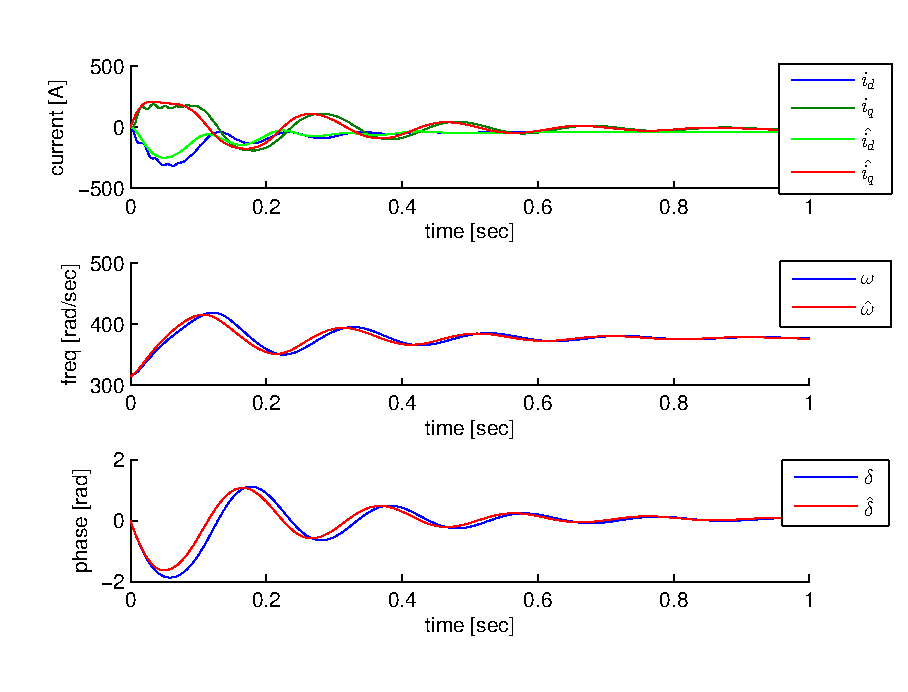
\includegraphics{sim5KWInfBus}

\caption{Simulation for infinite bus with single 5KW SG}
\label{fig:InfBusOne5KWSG}
\end{figure}

As shown in Figure \ref{fig:InfBusOne5KWSG}, simulations show that
for the 5KW SG, the behavior of the fourth order model and the reduced
model are almost the same. Although the currents at the reduced don't
have a ripple that the fourth order model has, both models converges
at the same rate with the same oscillations to the same equilibrium
point (The parameters for this simulation can be found at the appendix,
table \ref{table:5KWSG}). 

\subsection*{B. 1MW SG:}

\begin{figure}
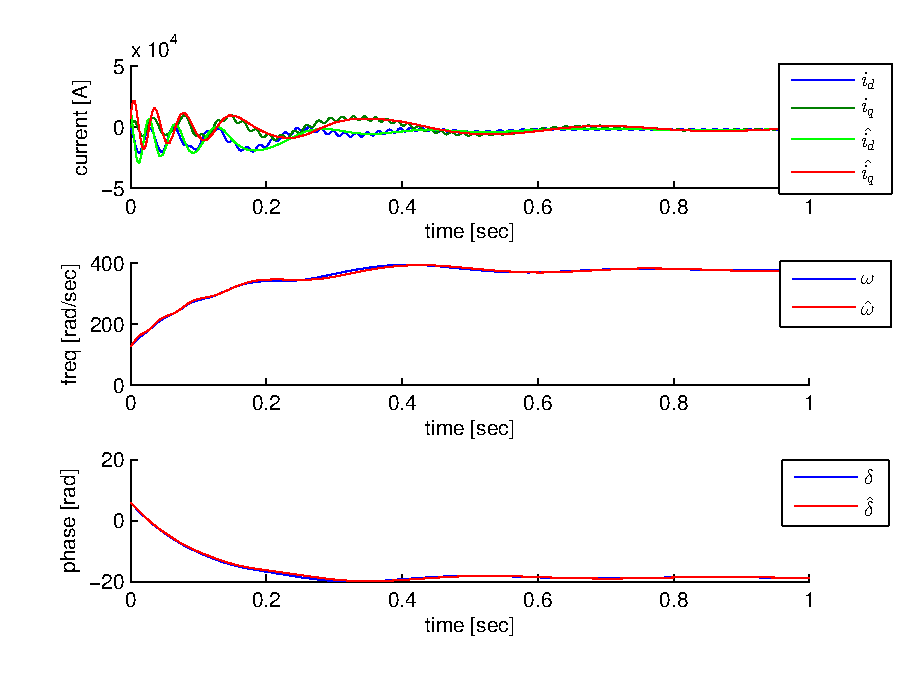
\includegraphics{sim1MWInfBus}

\caption{Simulation for infinite bus with single 1MW SG}
\label{fig:InfBusOne1MWSG}
\end{figure}

As shown in Figure \ref{fig:InfBusOne1MWSG}, simulations show that
for the 1MW SG, the behavior of the fourth order model and the reduced
model are still very similar. Although the fourth order model currents
are much rippled than the reduced model currents, both models converges
at the same rate with the same oscillations to the same equilibrium
point (The parameters for this simulation can be found at the appendix,
table \ref{table:1MWSG}). 

\subsection*{C. Non stable behavior for the reduced model:}

\begin{figure}
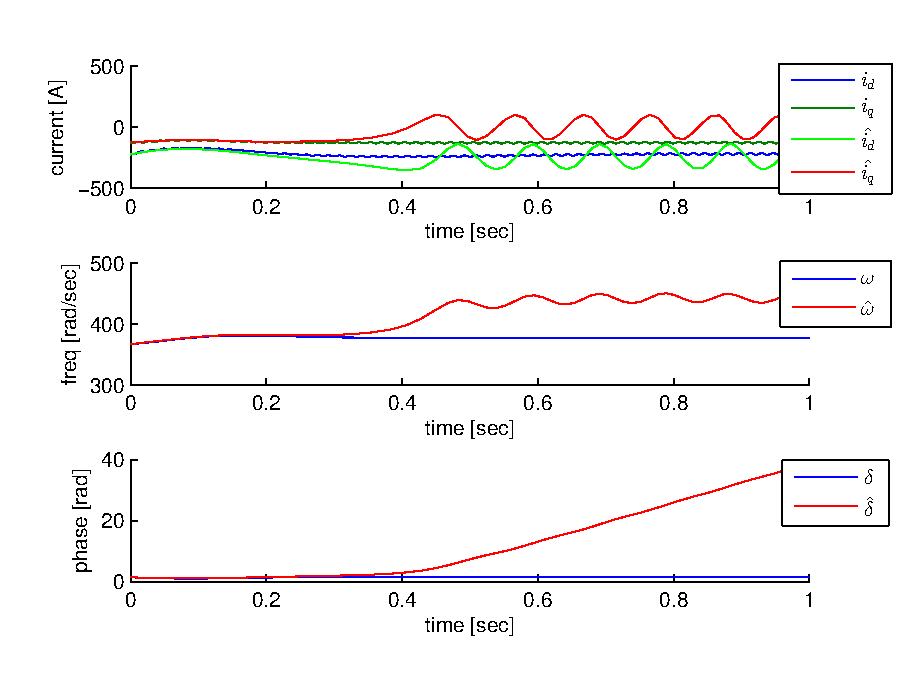
\includegraphics{simDiffBehavior1}

\caption{Simulation example that shows different behavior for the reduced model}
\label{fig:InfBusOne1DiffBehavior1}
\end{figure}

As shown in Figure \ref{fig:InfBusOne1DiffBehavior1}, simulations
show that for other parameters set (see appendix, table \ref{table:DifferentBehaviorParamsSetSG})
the behavior of the fourth order model and the reduced model is totally
different. while the four order model is stable (the eigenvalues of
the Jacobian around the equilibrium point are: 
\[
\left[\begin{array}{cccc}
-11.41+376.9i, & -11.41-376.9i, & -508+837i, & -508-837i\end{array}\right]
\]
, the reduced model is not stable (the eigenvalues of the Jacobian
around the equilibrium point are: $\left[\begin{array}{cc}
-14.6+9.4979i, & 6.1-9.4i\end{array}\right]$) .

\subsection*{D. Different region of attraction example :}

\begin{figure}
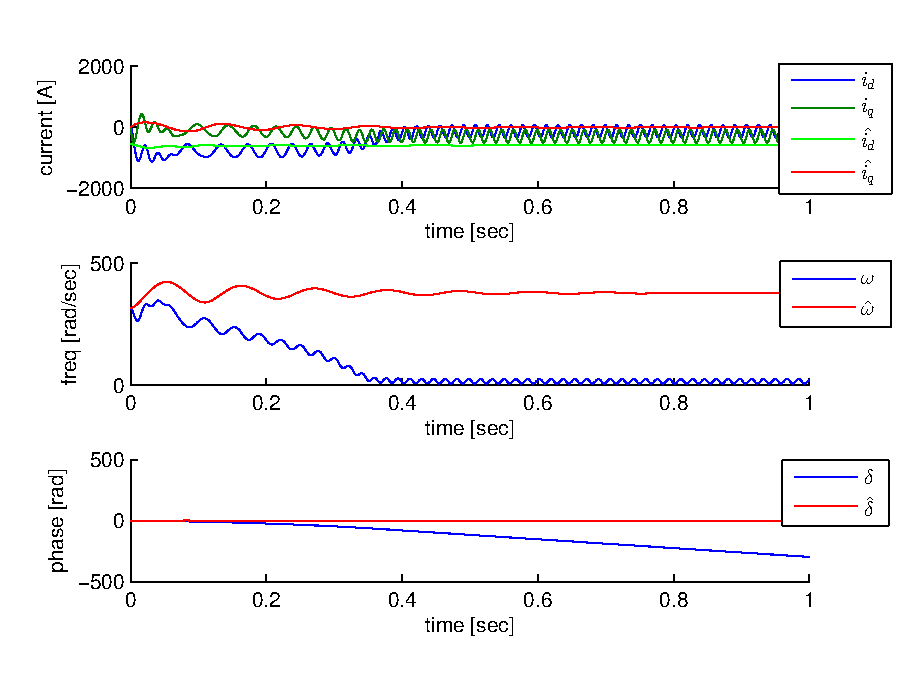
\includegraphics{simDiffRegionOFAttraction}

\caption{Simulation example that shows different behavior for the reduced model}
\label{fig:InfBusOne1DiffRegionOfAttraction}
\end{figure}

As shown in Figure \ref{fig:InfBusOne1DiffRegionOfAttraction}, simulations
show that for some parameters set (see appendix, table \ref{table:DifferentBehaviorParamsSetSG})
the initial condition of this simulation is within the region of attraction
of the reduced model, but outside the region of attraction of the
fourth model. That cause the fourth order model to diverge while the
reduce model converge to the equilibrium point. 



\chapter{Synchronization\label{cha:Synchronization}}

In this chapter, we show that microgid comprising of two identical
SGs, the synchronization manifold is locally exponentially stable.
First, we will rewrite the grid dynamics as synchronization error
dynamic, and equivalence SG dynamics. Then, we will prove that under
some conditions, the equivalence SG dynamics is globally exponentially
stable. Finally, we will use the main result from \citep{VincentBayuLaurent2016},
to show the stability of the system near the synchronization manifold.

\section{Modeling the synchronization problem:}

In order to show synchronization, it is convenient to use the following
notation:

\begin{equation}
\left\{ \begin{array}{c}
\dot{e}=F(e,x)\\
\dot{x}=G(e,x)
\end{array}\right.\label{eq:sync_sestem}
\end{equation}

Where 

\[
e\coloneqq\left[\begin{array}{c}
e_{d}\\
e_{q}\\
e_{\omega}\\
\delta
\end{array}\right]\coloneqq\left[\begin{array}{c}
i_{d1}-i_{d2}\\
i_{q1}-i_{q2}\\
\omega_{1}-\omega_{2}\\
\delta
\end{array}\right]
\]

\[
x\coloneqq\left[\begin{array}{c}
x_{d}\\
x_{q}\\
x_{\omega}
\end{array}\right]\coloneqq\left[\begin{array}{c}
i_{d1}+i_{d2}\\
i_{q1}+i_{q2}\\
\omega_{1}+\omega_{2}
\end{array}\right]
\]

Lets calculate the dynamics of the new notation:

from \eqref{eq:dynamics_whole}:

\[
\varLambda\dot{e}=\varLambda(\dot{z}_{1}-\dot{z}_{2})=\mathcal{A}(\omega_{1})z_{1}+T_{m}e_{3}-\mathcal{B}(\delta)z_{2}-\left(\mathcal{A}(\omega_{2})z_{2}+T_{m}e_{3}-\mathcal{B}(-\delta)z_{1}\right)
\]

\[
\begin{array}{ccc}
\varLambda\frac{d}{dt}\left[\begin{array}{c}
e_{d}\\
e_{q}\\
e_{\omega}\\
\delta
\end{array}\right] & = & \left[\begin{array}{c}
-R_{tot}(i_{d1}-i_{d2})+L_{s}(\omega_{1}i_{q1}-\omega_{2}i_{q2})\\
-L_{s}(\omega_{1}i_{d1}-\omega_{2}i_{d2})-R_{tot}(i_{q1}-i_{q2})-mi_{f}(\omega_{1}-\omega_{2})\\
mi_{f}(i_{q1}-i_{q2})-D_{p}(\omega_{1}-\omega_{2})\\
-(\omega_{1}-\omega_{2})
\end{array}\right]\\
 &  & +\left[\begin{array}{c}
R_{L}\cos(\delta)(i_{d1}-i_{d2})+R_{L}\sin(\delta)(i_{q1}+i_{q2})\\
R_{L}\cos(\delta)(i_{q1}-i_{q2})-R_{L}\sin(\delta)(i_{d1}+i_{d2})\\
0\\
0
\end{array}\right]
\end{array}
\]

Now, 

\[
(a+b)(x-y)+(a-b)(x+y)=2(ax-by)
\]

So

\[
\omega_{1}i_{q1}-\omega_{2}i_{q2}=\frac{1}{2}\left[(\omega_{1}+\omega_{2})(i_{q1}-i_{q2})+(\omega_{1}-\omega_{2})(i_{q1}+i_{q2})\right]=\frac{x_{w}e_{q}+e_{w}x_{q}}{2}
\]

and

\begin{equation}
\omega_{1}i_{d1}-\omega_{2}i_{d2}=\frac{x_{w}e_{d}+e_{w}x_{d}}{2}
\end{equation}

\[
\begin{array}{ccc}
\left[\begin{array}{cc}
\varLambda & 0\\
0 & 1
\end{array}\right]\dot{e} & = & \left[\begin{array}{cccc}
-R_{tot}+R_{L}\cos(\delta) & \frac{L_{s}}{2}x_{3} & \frac{L_{s}}{2}x_{2} & 0\\
-\frac{L_{s}}{2}x_{3} & -R_{tot}+R_{L}\cos(\delta) & -\frac{L_{s}}{2}x_{2}-mif & 0\\
0 & mi_{f} & -D_{p} & 0\\
0 & 0 & -1 & 0
\end{array}\right]e\\
 &  & +\left[\begin{array}{c}
R_{L}\sin(\delta)x_{2}\\
-R_{L}\sin(\delta)x_{1}\\
0\\
0
\end{array}\right]
\end{array}
\]

It is easy to see that $F(0,x)=0$, which shows that the manifold
$\epsilon=\left\{ \left[\begin{array}{c}
x\\
e
\end{array}\right]\in\mathbb{R}^{7}|e=0\right\} $ is invariant.

For the $x$ dynamics, we have:

\[
\varLambda\dot{x}=\varLambda(\dot{z}_{1}+\dot{z}_{2})=\mathcal{A}(\omega_{1})z_{1}+T_{m}e_{3}-\mathcal{B}(\delta)z_{2}+\mathcal{A}(\omega_{2})z_{2}+T_{m}e_{3}-\mathcal{B}(-\delta)z_{1}
\]

\[
\begin{array}{ccc}
\varLambda\frac{d}{dt}\left[\begin{array}{c}
x_{d}\\
x_{q}\\
x_{\omega}
\end{array}\right] & = & \left[\begin{array}{c}
-R_{tot}(i_{d1}+i_{d2})+L_{s}(\omega_{1}i_{q1}+\omega_{2}i_{q2})\\
-L_{s}(\omega_{1}i_{d1}+\omega_{2}i_{d2})-R_{tot}(i_{q1}+i_{q2})-mi_{f}(\omega_{1}+\omega_{2})\\
mi_{f}(i_{q1}+i_{q2})-D_{p}(\omega_{1}+\omega_{2})+2T_{m}
\end{array}\right]\\
 &  & +\left[\begin{array}{c}
-R_{L}\cos(\delta)(i_{d1}+i_{d2})-R_{L}\sin(\delta)(i_{q1}-i_{q2})\\
-R_{L}\cos(\delta)(i_{q1}+i_{q2})+R_{L}\sin(\delta)(i_{d1}-i_{d2})\\
0
\end{array}\right]
\end{array}
\]

Now, 

\[
(a+b)(x+y)+(a-b)(x-y)=2(ax+by)
\]

So

\[
\omega_{1}i_{q1}+\omega_{2}i_{q2}=\frac{1}{2}\left[(\omega_{1}+\omega_{2})(i_{q1}+i_{q2})+(\omega_{1}-\omega_{2})(i_{q1}-i_{q2})\right]=\frac{x_{w}x_{q}+e_{w}e_{q}}{2}
\]

and

\[
\omega_{1}i_{d1}-\omega_{2}i_{d2}=\frac{x_{w}x_{d}+e_{w}e_{d}}{2}
\]

\[
\varLambda\dot{x}=\left[\begin{array}{ccc}
-R_{tot}-R_{L}\cos(\delta) & \frac{L_{s}}{2}x_{\omega} & 0\\
-\frac{L_{s}}{2}x_{\omega} & -R_{tot}-R_{L}\cos(\delta) & -mif\\
0 & mi_{f} & -D_{p}
\end{array}\right]x+\left[\begin{array}{c}
\frac{L_{s}}{2}e_{\omega}e_{q}-R_{L}\sin(\delta)e_{q}\\
-\frac{L_{s}}{2}e_{\omega}e_{d}-R_{L}\sin(\delta)e_{d}\\
2T_{m}
\end{array}\right]
\]

For summery:

\[
\begin{array}{ccc}
\dot{e}=F(e,x) & = & \left[\begin{array}{cc}
\varLambda & 0\\
0 & 1
\end{array}\right]^{-1}\left[\begin{array}{cccc}
-R_{tot}+R_{L}\cos(\delta) & \frac{L_{s}}{2}x_{3} & \frac{L_{s}}{2}x_{2} & 0\\
-\frac{L_{s}}{2}x_{3} & -R_{tot}+R_{L}\cos(\delta) & -\frac{L_{s}}{2}x_{2}-mif & 0\\
0 & mi_{f} & -D_{p} & 0\\
0 & 0 & -1 & 0
\end{array}\right]e\\
 &  & +\left[\begin{array}{cc}
\varLambda & 0\\
0 & 1
\end{array}\right]^{-1}\left[\begin{array}{c}
R_{L}\sin(\delta)x_{2}\\
-R_{L}\sin(\delta)x_{1}\\
0\\
0
\end{array}\right]
\end{array}
\]

\[
\begin{array}{ccc}
\dot{x}=G(e,x) & = & \varLambda^{-1}\left[\begin{array}{ccc}
-R_{tot}-R_{L}\cos(\delta) & \frac{L_{s}}{2}x_{\omega} & 0\\
-\frac{L_{s}}{2}x_{\omega} & -R_{tot}-R_{L}\cos(\delta) & -mif\\
0 & mi_{f} & -D_{p}
\end{array}\right]x\\
 &  & +\varLambda^{-1}\left[\begin{array}{c}
\frac{L_{s}}{2}e_{\omega}e_{q}-R_{L}\sin(\delta)e_{q}\\
-\frac{L_{s}}{2}e_{\omega}e_{d}-R_{L}\sin(\delta)e_{d}\\
2T_{m}
\end{array}\right]
\end{array}
\]


\section{Globally exponentially stability of two synchronized generators:}

In this section, we provide sufficient conditions for the equilibrium
point which exist and located on the manifold $\epsilon=\left\{ \left[\begin{array}{c}
x\\
e
\end{array}\right]\in\mathbb{R}^{7}|e=0\right\} $\textbf{ }(chapter \ref{cha:equivalence_pont})\textbf{, }to be globally
exponential stable, for the dynamics of the two generators, assuming
that the system initial condition is located on the $\epsilon$ manifold
which is invariant manifold. This proof is very similar to section
3.5 at \citep{CaliiskanTabuada2014} 
\[
\dot{\tilde{x}}=\tilde{G}(\tilde{x})\coloneqq G(0,\tilde{x})=\varLambda^{-1}\left[\begin{array}{ccc}
-R_{tot}-R_{L} & \frac{L_{s}}{2}\tilde{x}_{\omega} & 0\\
-\frac{L_{s}}{2}\tilde{x}_{\omega} & -R_{tot}-R_{L} & -mif\\
0 & mi_{f} & -D_{p}
\end{array}\right]\tilde{x}+\varLambda^{-1}\left[\begin{array}{c}
0\\
0\\
2T_{m}
\end{array}\right]
\]

This system describes two generators when they have equal state and
no phase between each other.

Denote 

\[
A(\tilde{\omega})\coloneqq\left[\begin{array}{ccc}
-R_{tot}-R_{L} & \frac{L_{s}}{2}\tilde{\omega} & 0\\
-\frac{L_{s}}{2}\tilde{\omega} & -R_{tot}-R_{L} & -mif\\
0 & mi_{f} & -D_{p}
\end{array}\right],\tilde{\omega}\coloneqq\tilde{x}
\]

$\tilde{G}(\tilde{x})$ has at list one equilibrium point (\ref{cha:equivalence_pont})
$x^{0}=\left[\begin{array}{c}
x_{d}^{e}\\
x_{q}^{e}\\
\tilde{\omega}^{e}
\end{array}\right]$such:

\begin{equation}
\tilde{G}(x^{0})=0\rightarrow\varLambda^{-1}A(\tilde{\omega}^{e})\tilde{x}^{e}+\varLambda^{-1}\left[\begin{array}{c}
0\\
0\\
2T_{m}
\end{array}\right]=0\label{eq:G_at_equilibrium}
\end{equation}

Performing coordinations shift , in order to make the origin into
equilibrium point.

\[
\hat{x}\coloneqq\tilde{x}-\tilde{x}^{e}
\]

A natural Lyaponov function candidate is the total energy of the system:

\[
V(\hat{x})\coloneqq\frac{1}{2}L_{s}\left(\hat{x}_{d}^{2}+\hat{x}_{q}^{2}\right)+\frac{1}{2}J\tilde{\omega}^{2}=\frac{1}{2}\hat{x}^{T}\varLambda\hat{x}
\]

It is easy to see that:

\[
min(L_{s},J)|\hat{x}|{}^{2}\leq V(\hat{x})\leq max(L_{s},J)|\hat{x}|{}^{2}
\]

\[
\left|\frac{\partial V}{\partial\hat{x}}\right|=\left|\varLambda\hat{x}\right|\leq max(L_{s},J)\left|\hat{x}\right|
\]

Now, calculate $\dot{V}(\hat{x})$ in order to show that under some
conditions, $\dot{V}(\hat{x})\leq\alpha|\hat{x}|{}^{2}$, for some
$\alpha.$ This will prove that $\tilde{G}(\tilde{x})$ is globally
exponentially stable \citep{nonlinearSystemsSastry}.

\[
\dot{V}(\hat{x})=\left(\frac{\partial V}{\partial\hat{x}}\right)^{T}\dot{\hat{x}}
\]

\begin{equation}
\dot{\hat{x}}=\dot{\tilde{x}}=\varLambda^{-1}A(\tilde{\omega})\tilde{x}+\varLambda^{-1}\left[\begin{array}{c}
0\\
0\\
2T_{m}
\end{array}\right]\label{eq:x_hat_dynamic}
\end{equation}

Representing $A(\tilde{\omega})$ as a sum of a constant symmetric
matrix, constant skew symmetric matrix and a skew symmetric matrix
which depends on $\hat{\omega}$:

\[
R\coloneqq\left[\begin{array}{ccc}
-R_{tot}-R_{L} & 0 & 0\\
0 & -R_{tot}-R_{L} & 0\\
0 & 0 & -D_{p}
\end{array}\right]
\]

\[
J(\tilde{\omega}^{e})\coloneqq\left[\begin{array}{ccc}
0 & \frac{L_{s}}{2}\tilde{\omega}^{e} & 0\\
-\frac{L_{s}}{2}\tilde{\omega}^{e} & 0 & -mif\\
0 & mi_{f} & 0
\end{array}\right]
\]

\[
\Delta(\hat{\omega})\coloneqq\left[\begin{array}{ccc}
0 & \frac{L_{s}}{2}\hat{\omega} & 0\\
-\frac{L_{s}}{2}\hat{\omega} & 0 & 0\\
0 & 0 & 0
\end{array}\right]
\]

And now it is possible to represent the system dynamic:

\[
A(\tilde{\omega})\tilde{x}=\left[R+J(\tilde{\omega}^{0})+\Delta(\hat{\omega})\right](\hat{x}-\tilde{x}^{0})
\]

Combining this equation with \eqref{eq:G_at_equilibrium} and \eqref{eq:x_hat_dynamic}
obtains: 

\[
\dot{\hat{x}}=\varLambda^{-1}\left\{ \left[R+J(\tilde{\omega}^{e})+\Delta(\hat{\omega})\right]\hat{x}+\Delta(\hat{\omega})\tilde{x}^{e}\right\} 
\]

Calculate the derivative of the Lyponv function over the time: 

\[
\dot{V}(\hat{x})=\left(\varLambda\hat{x}\right)^{T}\dot{\hat{x}}=\hat{x}^{T}\varLambda^{T}\varLambda^{-1}\left\{ \left[R+J(\tilde{\omega}^{e})+\Delta(\hat{\omega})\right]\hat{x}+\Delta(\hat{\omega})\tilde{x}^{0}\right\} 
\]

Because $\varLambda$ is diagonal matrix, then $\varLambda^{T}\varLambda^{-1}=I$:

\[
\dot{V}(\hat{x})=\hat{x}^{T}\left[R+J(\tilde{\omega}^{e})+\Delta(\hat{\omega})\right]\hat{x}+\hat{x}^{T}\Delta(\hat{\omega})\tilde{x}^{e}
\]

\[
\dot{V}(\hat{x})=\hat{x}^{T}R\hat{x}+\hat{x}^{T}J(\tilde{\omega}^{e})\hat{x}+\hat{x}^{T}\Delta(\hat{\omega})\hat{x}+\hat{x}^{T}\Delta(\hat{\omega})\tilde{x}^{e}
\]

Because $J(\tilde{\omega}^{e})$ and $\Delta(\hat{\omega})$ are skew
symmetric matrices, it implies that $\hat{x}^{T}J(\tilde{\omega}^{e})\hat{x}=0$
and $\hat{x}^{T}\Delta(\hat{\omega})\hat{x}=0$ .

Calculating 

\[
\begin{array}{ccc}
\hat{x}^{T}\Delta(\hat{\omega})\tilde{x}^{0} & = & \left[\begin{array}{c}
\hat{x}_{d}\\
\hat{x}_{q}\\
\hat{\omega}
\end{array}\right]^{T}\left[\begin{array}{ccc}
0 & \frac{L_{s}}{2}\hat{\omega} & 0\\
-\frac{L_{s}}{2}\hat{\omega} & 0 & 0\\
0 & 0 & 0
\end{array}\right]\left[\begin{array}{c}
x_{d}^{e}\\
x_{q}^{e}\\
\tilde{\omega}^{0}
\end{array}\right]\\
 & = & \left[\begin{array}{c}
\hat{x}_{d}\\
\hat{x}_{q}\\
\hat{\omega}
\end{array}\right]^{T}\left[\begin{array}{ccc}
0 & 0 & \frac{L_{s}}{4}x_{q}^{e}\\
0 & 0 & -\frac{L_{s}}{4}x_{d}^{e}\\
\frac{L_{s}}{4}x_{q}^{e} & -\frac{L_{s}}{4}x_{d}^{e} & 0
\end{array}\right]\left[\begin{array}{c}
\hat{x}_{d}\\
\hat{x}_{q}\\
\hat{\omega}
\end{array}\right]\\
 & = & \hat{x}^{T}P\hat{x}
\end{array}
\]

Combining all this together, obtains: 

\[
\dot{V}(\hat{x})=\hat{x}^{T}\left[P+R\right]\hat{x}
\]

Where $P+R=\left[\begin{array}{ccc}
-R_{tot}-R_{L} & 0 & \frac{L_{s}}{4}x_{q}^{e}\\
0 & -R_{tot}-R_{L} & -\frac{L_{s}}{4}x_{d}^{e}\\
\frac{L_{s}}{4}x_{q}^{e} & -\frac{L_{s}}{4}x_{d}^{e} & -D_{p}
\end{array}\right]$. Calculating the eigenvalues of $P+R$:

\[
det\left(P+R-\lambda I\right)=\begin{vmatrix}-R_{tot}-R_{L}-\lambda & 0 & \frac{L_{s}}{4}x_{q}^{e}\\
0 & -R_{tot}-R_{L}-\lambda & -\frac{L_{s}}{4}x_{d}^{e}\\
\frac{L_{s}}{4}x_{q}^{e} & -\frac{L_{s}}{4}x_{d}^{e} & -D_{p}-\lambda
\end{vmatrix}
\]

\[
=\left(-R_{tot}-R_{L}-\lambda\right)\left[\left(-R_{tot}-R_{L}-\lambda\right)\left(-D_{p}-\lambda\right)+\frac{L_{s}^{2}}{16}\left(x_{d}^{e}\right)^{2}\right]+\frac{L_{s}}{4}x_{q}^{e}\left[-\left(-R_{tot}-R_{L}-\lambda\right)\frac{L_{s}}{4}x_{q}^{e}\right]
\]

\[
=\left(R_{tot}+R_{L}+\lambda\right)\left[\left(R_{tot}+R_{L}+\lambda\right)\left(D_{p}+\lambda\right)-\frac{L_{s}^{2}}{16}\left[\left(x_{q}^{e}\right)^{2}+\left(x_{d}^{e}\right)^{2}\right]\right]=\left(R_{tot}+R_{L}+\lambda\right)\pi(\lambda)
\]

The first eigenvalue of $P+R$ is $\lambda_{1}=-\left(R_{tot}+R_{L}\right)$
which is negative. $\pi(\lambda)=\lambda^{2}+\lambda\left(R_{tot}+R_{L}+D_{p}\right)+\left(R_{tot}+R_{L}\right)D_{p}-\frac{L_{s}^{2}}{16}\left[\left(x_{q}^{e}\right)^{2}+\left(x_{d}^{e}\right)^{2}\right]$

\[
\lambda_{2,3}=-\frac{R_{tot}+R_{L}+D_{p}}{2}\pm\frac{\sqrt{4\left(R_{tot}+R_{L}-D_{p}\right)^{2}+2\left(R_{tot}+R_{L}\right)D_{p}+L_{s}^{2}\left(\left(x_{q}^{e}\right)^{2}+\left(x_{d}^{e}\right)^{2}\right)}}{4}
\]

All eigenvalues are real numbers. The condition which implies that
all the eigenvalues will be negative is:

\[
-\frac{R_{tot}+R_{L}+D_{p}}{2}+\frac{\sqrt{4\left(R_{tot}+R_{L}-D_{p}\right)^{2}+2\left(R_{tot}+R_{L}\right)D_{p}+L_{s}^{2}\left(\left(x_{q}^{e}\right)^{2}+\left(x_{d}^{e}\right)^{2}\right)}}{4}<0
\]

\[
4\left(R_{tot}+R_{L}+D_{p}\right)^{2}>4\left(R_{tot}+R_{L}-D_{p}\right)^{2}++L_{s}^{2}\left(\left(x_{q}^{e}\right)^{2}+\left(x_{d}^{e}\right)^{2}\right)
\]

Which leads to the following condition:

\begin{equation}
16\left(R_{tot}+R_{L}\right)D_{p}>L_{s}^{2}\left(\left(x_{q}^{e}\right)^{2}+\left(x_{d}^{e}\right)^{2}\right)\label{eq:condition_for_stable_G}
\end{equation}

If this condition \eqref{eq:condition_for_stable_G} holds, then $\dot{V}(\hat{x})<min(\lambda_{i})|\hat{x}|^{2},i\in\{1,2,3\}$.
This proves that this system is globally exponentially stable. That
implies that $\tilde{x}^{e}$ is the only equilibrium point of $\tilde{G}(\tilde{x})$,
hence the original system has only one equilibrium point on the subspace
where $z_{1}=z_{2}$ and $\delta=0$. In addition it always has another
equilibrium point on the surface $z_{1}=z_{2}$ and $\delta=\pi$.

\section{Synchronization theorem:}

In this section, we prove that if the initial state of the two generators
are sufficiently close to each other, i.e $|e(0)|$ is small, then,
under some conditions, the two generators will synchronize, meaning
that $lim_{t\to\infty}e(t)=0$.

For this, we use the result from \citep{VincentBayuLaurent2016}.

First, 

\begin{equation}
\frac{\partial F(e,x)}{\partial e}(0,x)=\left[\begin{array}{cccc}
-\frac{R_{s}}{L_{s}} & \frac{x_{\omega}}{2} & \frac{x_{q}}{2} & -\frac{R_{L}}{L_{s}}x_{q}\\
-\frac{x_{\omega}}{2} & -\frac{R_{s}}{L_{s}} & -\frac{x_{d}}{2}{}_{2}-\frac{mif}{L_{s}} & \frac{R_{L}}{L_{s}}x_{d}\\
0 & \frac{mi_{f}}{J} & -\frac{D_{p}}{J} & 0\\
0 & 0 & -1 & 0
\end{array}\right]\label{eq:div_of_F}
\end{equation}

The requirement (2) at \citep{VincentBayuLaurent2016} namely that
matrix \eqref{eq:div_of_F} should by uniformly bounded (in norm on
the manifold $\epsilon=\left\{ \left[\begin{array}{c}
x\\
e
\end{array}\right]\in\mathbb{R}^{7}|e=0\right\} $is \uline{not satisfied}, because of the presences of $x_{w},x_{q},x_{d}$
in the matrix. However, it can be shown by energy methods that regardless
of the initial state, the state of this system will be eventually
contained in a certain bounded set (that depends on the parameters)
and than $\frac{\partial F(}{\partial e}(0,x)$ is clearly bounded
in this bounded subset of the state space.

The requirement (3) in \citep{VincentBayuLaurent2016} is satisfied
as showed. Additionally we showed at the last section that $\tilde{G}(\tilde{x})$
is globally exponentially stable with equilibrium $x^{e}$. We will
show that our system \eqref{eq:sync_sestem} is UES-TL (Uniform exponential
stability for the transversally linear system), as it defines at \citep{VincentBayuLaurent2016}. 

we need to show that the system 

\[
\dot{\tilde{e}}=\frac{\partial F}{\partial e}(0,\tilde{x})\tilde{e}
\]

is stable, where $\tilde{x}(t)$ generated by the dynamics 
\[
\tilde{x}=\tilde{G}(\tilde{x})
\]
 which we showed that it globally exponentially stable (and $lim_{t\to\infty}\tilde{x}(t)=0$).
In order to have the UES-TL property, we will demand that $\tilde{G}(0)$
is a Hurwitz matrix. We need to show that there exist constants $k$,$r$
and $\lambda$ such for all $\left|e^{e}\right|\leq r$ and for all
$x^{e}$.

\[
\left|e(t)\right|\leq k\left|e_{0}\right|exp(-\lambda t)
\]

In other words, we need to show that if LTV (linear time varying system),
which it matrix converges exponentially to a stable matrix, then the
LTV system is exponentially stable. this theorem is known (\citep{SchovanecGilliam1999}),
but for the clearance of the reading, we will repeat the proof:

\subparagraph*{Theorem:}

Let $A$ be a constant matrix with $Re\{\sigma(A)\}<0$ and let $C$
be a continuous matrix valued function on the function on the interval
$[0,\infty)$. Supposed that 

\[
\intop_{0}^{\infty}\left|C(t)\right|dt=M<\infty
\]

Then, the solution of 

\begin{equation}
\dot{x}(t)=[A+C(t)]x(t)\label{eq:LTV_dynamics}
\end{equation}

is globally exponentially stable.

\subparagraph*{Proof:}

Suppose that x(t) is a solution of \eqref{eq:LTV_dynamics} with $x(0)=x^{e}$.
We have 

\[
\dot{x}(t)-Ax(t)=C(t)x(t)
\]

If we multiply this equation through by the integrating factor (matrix)
$e^{-At}$, we get 

\[
\frac{d}{dt}\left(e^{-At}x(t)\right)=e^{-At}C(t)x(t)
\]

Integrating the last equation from $0$ to $t$ gives:

\[
e^{-At}x(t)-x(0)=\intop_{0}^{t}e^{-As}C(s)x(s)ds
\]

This gives us the formula

\begin{equation}
x(t)=e^{At}x(0)\intop_{0}^{t}e^{A(t-s)}C(s)x(s)ds\label{eq:LTV_integralForm}
\end{equation}

Since $Re\{\sigma(A)\}<0$, we can find constants $\sigma<0$ and
$K>0$ such that $\left|e^{At}\right|\leq Ke^{\sigma t},\;t\geq0$ 

using this estimates and taking norms in \eqref{eq:LTV_integralForm}
we get 

\[
\left|x(t)\right|\leq K\left|x^{e}\right|e^{\sigma t}+\intop_{0}^{t}Ke^{\sigma(t-s)}\left|C(s)\right|\left|x(s)\right|ds
\]

Multiply this through by $e^{-\sigma t}$ to get

\[
e^{-\sigma t}\left|x(t)\right|\leq K\left|x^{e}\right|+\intop_{0}^{t}K\left|C(s)\right|e^{-\sigma s}\left|x(s)\right|ds
\]

By applying Gronwall's inequality:

\[
e^{-\sigma t}\left|x(t)\right|\leq K\left|x^{e}\right|+\intop_{0}^{t}K^{2}\left|x^{e}\right|\left|C(s)\right|exp\left[\intop_{s}^{t}K\left|C(u)\right|du\right]ds
\]
For any $0\le s\le t$, we must have $\intop_{s}^{t}\left|C(u)\right|du\le\intop_{0}^{\infty}\left|C(t)\right|dt=M$.
Thus, 
\[
exp\left[\intop_{s}^{t}K\left|C(u)\right|du\right]\le e^{KM}
\]
Applying this gives

\[
e^{-\sigma t}\left|x(t)\right|\leq K\left|x^{e}\right|+e^{KM}K^{2}\left|x^{e}\right|\intop_{0}^{t}\left|C(s)\right|ds\le K\left|x^{e}\right|+e^{KM}K^{2}M
\]

So 

\[
\left|x(t)\right|\leq e^{\sigma t}C^{e}\left|x^{e}\right|,\quad\sigma<0
\]

This proves that our system \eqref{eq:sync_sestem}is UES-TL. By applying
the main result of \citep{VincentBayuLaurent2016}, proves that this
system is TULES-NL (Transversal uniform local exponential stable).
That means that there exist strictly positive real numbers $r$, $k$
and $\lambda$such for all $(e^{e},x^{e},t)$ in $B_{e}(r)\times R^{3}\times\mathbb{R}_{\geq0}$
, $e(t)$ satisfies $\left|e(t)\right|\leq k\left|e^{e}\right|exp(-\lambda t)$.
Namely the manifold $\epsilon$ is exponentially stable for the system
\eqref{eq:sync_sestem}, locally in $e$,uniformly in $x$.


\bibliography{references}
\bibliographystyle{abbrvnat}

\appendix

\chapter{Synchronous generator parameters\label{chap:Appendix}}

\subsection*{5 KW SG}

The parameters of 5KW SG are taken from \cite{Brown2015}

\begin{table}[H]
\begin{tabular}{|c|c|}
\hline 
Variable & Value\tabularnewline
\hline 
\hline 
$J$ & $0.2\qquad[kgm^{2}]$\tabularnewline
\hline 
$D_{p}$ & $1.7\qquad\left[\frac{Joule}{sec}\right]$\tabularnewline
\hline 
$R_{s}$ & $0.152\qquad\left[\Omega\right]$\tabularnewline
\hline 
$L_{s}$ & $4.4\qquad\left[mH\right]$\tabularnewline
\hline 
$mi_{f}$ & $1.05\qquad\left[Vsec\right]$\tabularnewline
\hline 
$\omega_{g}$ & $60\cdotp2\cdotp\pi\qquad\left[\frac{rad}{sec}\right]$\tabularnewline
\hline 
$V$ & $330\qquad\left[V\right]$\tabularnewline
\hline 
$P_{m}$ & $5\qquad\left[kW\right]$\tabularnewline
\hline 
\end{tabular}\caption{Parameters for 5KW SG}
\label{table:5KWSG}
\end{table}


\subsection*{1 MW SG}

The parameters of 1MW SG are taken from \cite{Brown2015}

\begin{table}[H]
\begin{tabular}{|c|c|}
\hline 
Variable & Value\tabularnewline
\hline 
\hline 
$J$ & $40.05\qquad[kgm^{2}]$\tabularnewline
\hline 
$D_{p}$ & $337\qquad\left[\frac{Joule}{sec}\right]$\tabularnewline
\hline 
$R_{s}$ & $0.4\qquad\left[m\Omega\right]$\tabularnewline
\hline 
$L_{s}$ & $18\qquad\left[mH\right]$\tabularnewline
\hline 
$mi_{f}$ & $1.79\qquad\left[Vsec\right]$\tabularnewline
\hline 
$\omega_{g}$ & $60\cdotp2\cdotp\pi\qquad\left[\frac{rad}{sec}\right]$\tabularnewline
\hline 
$V$ & $563\qquad\left[V\right]$\tabularnewline
\hline 
$P_{m}$ & $1\qquad\left[MW\right]$\tabularnewline
\hline 
\end{tabular}\caption{Parameters for 1MW SG}
\label{table:1MWSG}
\end{table}


\subsection*{Example for SG parameters which leads to different behavior for the
reduced model}

This set of parameters shows different behavior of the whole model
and for the improved swing equation model. This set of parameters
is basically the 5KW SG parameters set which connected to grid with
lower voltage and fed by $50$ {[}KW{]} prime mover. 

\begin{table}[H]
\begin{tabular}{|c|c|}
\hline 
Variable & Value\tabularnewline
\hline 
\hline 
$J$ & $0.2\qquad[kgm^{2}]$\tabularnewline
\hline 
$D_{p}$ & $1.7\qquad\left[\frac{Joule}{sec}\right]$\tabularnewline
\hline 
$R_{s}$ & $0.152\qquad\left[\Omega\right]$\tabularnewline
\hline 
$L_{s}$ & $4.4\qquad\left[mH\right]$\tabularnewline
\hline 
$mi_{f}$ & $1.05\qquad\left[Vsec\right]$\tabularnewline
\hline 
$\omega_{g}$ & $60\cdotp2\cdotp\pi\qquad\left[\frac{rad}{sec}\right]$\tabularnewline
\hline 
$V$ & $200\qquad\left[V\right]$\tabularnewline
\hline 
$P_{m}$ & $50\qquad\left[kW\right]$\tabularnewline
\hline 
\end{tabular}\caption{Parameters for SG which leads to different behavior for the reduced
model}
\label{table:DifferentBehaviorParamsSetSG}
\end{table}


\subsection*{Example for SG parameters which leads to different behavior for the
reduced model}

This set of parameters shows different region of attraction of the
whole model and for the improved swing equation model. This set of
parameters is basically the 5KW SG parameters set with stronger $i_{f}$
(or stronger permanent magnet).

\begin{table}[H]
\begin{tabular}{|c|c|}
\hline 
Variable & Value\tabularnewline
\hline 
\hline 
$J$ & $0.2\qquad[kgm^{2}]$\tabularnewline
\hline 
$D_{p}$ & $1.7\qquad\left[\frac{Joule}{sec}\right]$\tabularnewline
\hline 
$R_{s}$ & $0.152\qquad\left[\Omega\right]$\tabularnewline
\hline 
$L_{s}$ & $1.05\qquad\left[mH\right]$\tabularnewline
\hline 
$mi_{f}$ & $3.5\qquad\left[Vsec\right]$\tabularnewline
\hline 
$\omega_{g}$ & $60\cdotp2\cdotp\pi\qquad\left[\frac{rad}{sec}\right]$\tabularnewline
\hline 
$V$ & $330\qquad\left[V\right]$\tabularnewline
\hline 
$P_{m}$ & $5\qquad\left[kW\right]$\tabularnewline
\hline 
\end{tabular}\caption{Parameters for SG which leads to different region of attraction}
\label{table:DifferentRegionOfAttraction}
\end{table}



\newpage{}

\end{document}
